% ****** Start of file apssamp.tex ******
%
%   This file is part of the APS files in the REVTeX 4.1 distribution.
%   Version 4.1r of REVTeX, August 2010
%
%   Copyright (c) 2009, 2010 The American Physical Society.
%
%   See the REVTeX 4 README file for restrictions and more information.
%
% TeX'ing this file requires that you have AMS-LaTeX 2.0 installed
% as well as the rest of the prerequisites for REVTeX 4.1
%
% See the REVTeX 4 README file
% It also requires running BibTeX. The commands are as follows:
%
%  1)  latex apssamp.tex
%  2)  bibtex apssamp
%  3)  latex apssamp.tex
%  4)  latex apssamp.tex
%
\documentclass[%
 reprint,
%superscriptaddress,
%groupedaddress,
%unsortedaddress,
%runinaddress,
%frontmatterverbose, 
%preprint,
%showpacs,preprintnumbers,
%nofootinbib,
%nobibnotes,
%bibnotes,
 amsmath,amssymb,
 aps,
%pra,
%prb,
%rmp,
%prstab,
%prstper,
%floatfix,
]{revtex4-1}

\usepackage{graphicx}% Include figure files
\usepackage{multirow}
\usepackage{colortbl}
\usepackage[]{units}
\usepackage{siunitx}
\usepackage{pdfpages}

\usepackage{hyperref}
\usepackage{url}
\usepackage{graphicx}
\usepackage{dcolumn}% Align table columns on decimal point
\usepackage{bm}% bold math
%\usepackage{hyperref}% add hypertext capabilities
%\usepackage[mathlines]{lineno}% Enable numbering of text and display math
%\linenumbers\relax % Commence numbering lines

%\usepackage[showframe,%Uncomment any one of the following lines to test 
%%scale=0.7, marginratio={1:1, 2:3}, ignoreall,% default settings
%%text={7in,10in},centering,
%%margin=1.5in,
%%total={6.5in,8.75in}, top=1.2in, left=0.9in, includefoot,
%%height=10in,a5paper,hmargin={3cm,0.8in},
%]{geometry}

\begin{document}

\preprint{APS/123-QED}

\title{Development of the Timing System for the Bunch-to-Bucket Transfer between the FAIR Accelerators}% Force line breaks with \\

\author{J. Bai$^{1,2}$}
 \altaffiliation[Email: ]{baijiaoni1314@gmail.com}%Lines break automatically or can be forced with \\
\author{T. Ferrand$^{1,3}$, O. Kester$^{1,4}$, D. Ondreka$^{1}$, D. Beck$^{1}$, C. Prados$^{1,?}$}%

\affiliation{
1. GSI Helmholtzzentrum f$\ddot{u}$r Schwerionenforschung, 64291 Darmstadt, Germany
\\2. IAP, Goethe University Frankfurt am Main, 60439 Frankfurt am Main, Germany \\
3. TEMF, Technique University Darmstadt, 64291 Darmstadt, Germany\\
4. TRIUMF, 4004 Wesbrook Mall Vancouver, BC V6T 2A3 Canada }


\begin{abstract} 
The Facility for Antiproton and Ion Research (FAIR) project is aiming at providing high-energy beams of ions of all elements
from hydrogen to uranium, as well as antiprotons and rare isotopes with high intensities. The existing accelerator facility of GSI  Helmholtz center for Heavy Ion Research GmbH (short: GSI) and the future FAIR facility employ a variety of circular accelerators like heavy ion synchrotrons (the SIS18 and the
SIS100) and storage rings (the experimental storage ring ESR, the CRYRING@ESR, the collector ring CR and the high energy storage ring HESR) for the preparation of secondary beams and experiments. Bunches are required to be transferred into rf buckets among GSI and FAIR ring accelerators for different purposes. All this imposes new requirements on the bunch-to-bucket transfer system. These requirements include the bunch-to-bucket transfer between two rings with an arbitrary ratio in their circumference, two synchronization methods (the phase shift method and the frequency beating method), the required bunch-to-bucket transfer time \SI{10}{\ms}, the tolerable bunch-to-bucket injection center mismatch less than $\pm1^\circ$ and the primary beam transfer as well as the secondary beam. In order to fulfill these requirements, a completely new and unique FAIR bunch-to-bucket transfer system will be developed. The presentation of the concept of the system and the systematic investigation from timing perspective are the purpose of this paper. The concept and basic procedure of the system first of all are presented. Afterwards, a systematic investigation from the beam dynamics, timing requirement of the transfer and kicker trigger perspectives is analyzed. Finally, the application of the system for all FAIR use cases with the frequency beating method is summarized.


\begin{description}
%\item[Usage]
%Secondary publications and information retrieval purposes.
\item[PACS numbers]
29.20.D-. 29.27.Ac. 07.05.Dz

\end{description}
\end{abstract}

\pacs{Valid PACS appear here}% PACS, the Physics and Astronomy
                             % Classification Scheme.
%\keywords{Suggested keywords}%Use showkeys class option if keyword
                              %display desired
\maketitle

%\tableofcontents

\section{\label{sec:introduction}INTRODUCTION}
FAIR is a new international accelerator facility under construction at GSI. It is aiming at providing high-energy beams of ions of all elements from hydrogen to uranium with high intensities, as well as beams of rare isotopes and of antiprotons~\cite{eschke_international_2005, noauthor_fair_2011}. The FAIR facility in its start version will consist of three circular accelerators (short: ring), the SIS100, the CR and the HESR. In addition, the GSI accelerator facility complements the planned accelerators of FAIR, which comprises the SIS18, the ESR and the CRYRING. Bunches are required to be transferred into radio frequency (rf) buckets among GSI and FAIR rings by the so-called bunch-to-bucket (B2B) transfer method. An implementation of the B2B transfer from the SIS18 to the ESR exists, the phase difference between the two rf systems is measured based on the direct transmission of the analog rf signals of the two rings to a central station. However the direct transmission is undesired for the new FAIR accelerator complex, which will be around six times larger than the existing GSI site. In order to avoid the direct transmission, a center clock can be used, which provides a reference clock to the rf systems of the two rings. The phase difference between the rf system and the reference clock is measured at each ring locally and the measurement results are transferred to a central station to calculate the phase difference. Coincidentally, the FAIR Bunchphase Timing System (BuTiS)~\cite{moritz_butisdevelopment_2006} can provide such a reference clock for the B2B transfer, which serves as a campus-wide clocks distribution system for the low level radio frequency (LLRF) system ~\cite{klingbeil_new_2011} with sub nanosecond resolution and stability over distances of several hundred meters~\cite{moritz_f-cs-rf-14e_2012}. In addition, the FAIR new timing system, the General Machine Timing (GMT) system~\cite{beck_general_2013}, is based on the sub-nanosecond synchronization White Rabbit (WR) network~\cite{beck_white_2011}, which can transfer the measurement results deterministically. Therefore, a new FAIR B2B transfer system based on the GMT system, the LLRF system and the BuTiS is required. 

The concept of the B2B transfer was first introduced in the early 1980s at the European Organization for Nuclear Research (CERN) for the beam transfer from the Proton Synchrotron Booster (PSB) to the PS~\cite{garoby_cern-ps-rf-note-84-6_1984} and the B2B transfer has been used for almost three decades around the world. The FAIR B2B transfer is comparable with the CERN B2B transfer. At CERN, primary beams of ions of all elements can be transferred among rings as at FAIR, e.g. the Large Hadron Collider (LHC) is supplied with \SI{7}{TeV} high energy proton beams from the injector chain PSB - Proton Synchrotron (PS) -  Super Proton Synchrotron (SPS) and with \SI{2.76}{TeV/u} high energy heavy ion beams from the injection chain Low Energy Ion Ring (LEIR) - PS - SPS  ~\cite{noauthor_cern_nodate}. In addition, the CERN B2B transfer system transfers the secondary beams to rf buckets, e.g. a proton beam that comes from the PS is fired into an antiproton (pbar) target to produce the antiproton beam and the antiproton beam is transferred into Antiproton Decelerator (AD). However, the CERN B2B transfer is based on the direct transmission of the analog signal (e.g. the revolution frequency signal of the target ring) from the target ring to the source ring as the GSI existing B2B transfer implementation, which is used for the bucket counting and synchronization. The instability of every analog signal transmission delay along coaxial cables or optical fibers (e.g. the thermal drift) is compensated individually. In order to synchronize two rings, the beam of the source ring is moved to an off-momentum position by adjusting the cavities frequency (the magnetic field is constant). A periodic beating of the phase between the revolution signals of the two rings is observed. The relative azimuthal position between the two rings is measured and the beam is moved back to the reference momentum when it reaches the correct azimuth ~\cite{damerau_lecture_2017}. The synchronization process between the PS and the SPS takes about \SI{50}{\ms}~\cite{ferrand_cern-acc-note-2015-0025_2015} and that between the SPS and the LHC takes about \SI{30}{\ms}~\cite{baudrenghien_sps_1998}. 

The FAIR B2B transfer system avoids the direct analog signal transmission. It makes use of not only the mentioned azimuthal position correction as CERN to realize the synchronization process, but also the automatically azimuthal position correction with the help of the circumference ratio between two rings, which decreases the time duration of the synchronization process.   

In the following section, the requirements for the FAIR B2B transfer system is listed. In Sec. ~\ref{concept} the concept of the FAIR B2B transfer system is introduced together with the basic procedure. The FAIR B2B transfer system focus first of all on the transfer from the SIS18 to the SIS100. Hence, the Sec. ~\ref{dynamics} is concerned with the analysis of the two synchronization methods from the beam dynamics for the B2B transfer from the SIS18 to the SIS100. In Sec.~\ref{timing}, the timing constraints of the system is presented. Afterwards the application of the system for FAIR use cases is presented in Sec. ~\ref{application}.




\section{\label{concept}CONCEPT OF THE FAIR B2B TRANSFER SYSTEM}
The new FAIR B2B transfer system relies on the FAIR technical basis, the FAIR timing and control system and the low-level radio frequency (LLRF) system. The FAIR control system takes advantage of several collaborations with CERN by using, adapting and improving framework solutions like the settings management framework LSA, the front-end software framework FESA and the WR based timing system as core components ~\cite{huhmann_fair_2013}. The General Machine Timing (GMT) system synchronizes all Front End Controllers (FEC) with nanosecond accuracy over the whole FAIR campus and distributes timing messages to all FECs via the reliable and robust WR network and controls all FECs to execute real-time actions at a designated time ~\cite{beck_new_2012}. The GMT system mainly consists of a data master (DM), the WR network and FECs. The DM defines the accelerator schedule. The Scalable Control Unit (SCU) ~\cite{kaiser_f-tn-c-008e_2014} is a new generation of the standard FEC for the FAIR control system, which provides a compact and flexible solution for controlling all types of accelerator equipment. For the synchronization of the LLRF system, the GMT system is complemented and linked to the Bunch Phase Timing System (BuTiS) ~\cite{moritz_butisdevelopment_2006, moritz_f-cs-rf-14e_2012}, which serves as a campus-wide clocks distribution system with sub nanosecond resolution and stability over distances of several hundred meters. The LLRF system synchronizes cavities in every ring by the reference rf signal distribution system (short: rf system) ~\cite{klingbeil_detailed_2013}. 

In order to complete the B2B transfer, first of all, the rf systems of the source and target rings must be correctly phase aligned. Secondly, the trigger for the extraction and injection kicker magnets must be synchronized with the beam. Finally the time point of the actual beam injection into the target ring must be indicated to enable beam instrumentation devices to measure the properties and the behavior of the beam directly after the injection. In the following, the realization of these three functionalities will be presented. For the B2B transfer, there is a so-called “B2B transfer master“, which is responsible for the data collection of two rings, the data calculation, the data redistribution and the B2B transfer status check. For the sake of simplicity, the source ring works as the B2B transfer master.

\subsection{Phase alignment}
In order to realize the phase alignment, the phase difference $\Delta \phi$ between the two rf systems of two rings must be obtained. The phase difference is indirectly measured via a FAIR campus wide distributed reference signal synchronized with BuTiS clocks. 
\begin{eqnarray}
\begin{aligned}
	\Delta \phi&=(\Delta \phi_1-\Delta \phi_2) \mod 2\pi\\
&=[2\pi(f_1-f_\mathit{ref})t+\phi_1]\\
&-[2\pi(f_2-f_\mathit{ref})t+\phi_2] \mod 2\pi \\
&=[2\pi(f_1-f_2)t+\phi_1-\phi_2] \mod 2\pi
\end{aligned}
\end{eqnarray}

where $\phi_1$ and $\phi_2$ are the initial phases of the two rf systems of the source and target rings, $f_1$ and $f_2$ the frequencies of the two rf systems, $f_\mathit{ref}$ the frequency of the reference signal and $\Delta \phi_1$ and $\Delta \phi_2$ the phase difference between the two rf systems and the reference signal. 

For the phase difference, there are two scenarios according to the relation between $f_1$ and $f_2$. When $f_1$ equals to $f_2$, $\Delta \phi$ is constant. In order to change the phase difference for the phase alignment, the phase of either (or both) rf system must be shifted by modulating the frequency of the rf system away from the reference value for a specific period of time and then modulating back. This is called ``phase shift``.

When $f_1$ and $f_2$ are slightly different, $\Delta \phi$ is a periodic function whose rate is the difference between two frequencies. This is called ``frequency beating``. The periodically variable rate is called the ``beating frequency``, $\Delta f=|f_1-f_2|$. The beating period is defined as a period of time for the periodical variation, namely $1/\Delta f$. Within one beating period, there exists a time point, which corresponds to a correct phase difference between the two rf systems, namely the phase alignment. 

The phase alignment is realized based on two identical or two slightly different frequencies. These two frequencies are called ``synchronization frequencies``, denoted as $f_\mathit{syn}^{X}$, where X indicates the ring. The phase difference between two synchronization frequency is denoted as $\Delta \phi_\mathit{syn}$. The number of circulating buckets is determined by the harmonic number and the cavity rf frequency is the harmonic number times of the revolution frequency. The cavity rf frequency is denoted as $f_\mathit{rf}^{X}$ and the revolution frequency $f_\mathit{rev}^{X}$. The FAIR LLRF system produces the revolution frequency as the $1^{st}$ harmonic and supports not only the integer multiple but also the fractional multiple of the revolution frequency. For all FAIR use cases, two synchronization frequencies are an integer multiple of the same or slightly different derived rf frequencies, which are the fraction of the revolution frequencies.
\begin{equation}
f_\mathit{syn}^{X}= Y\cdot f_\mathit{rev}^{X}/m
\label{syn_form}
\end{equation}
where $f_\mathit{rev}^{X}/m$ represents the fraction of the revolution frequency and both $m$ and $Y$ are positive integers, which are determined by the circumference ratio and the harmonic numbers. 

For FAIR use cases with an integer ratio in their circumference, there is an integer multiple relationship between two revolution frequencies. In this case, two identical synchronization frequencies are integer times of the revolution frequencies, namely $m=1$ in eq. ~\ref{syn_form}. For example, the $H^{+}$ B2B transfer from the SIS18 to the SIS100 has $f_{\mathit{syn}}^{SIS100}=5f_{\mathit{rev}}^{SIS100}$ and $f_{\mathit{syn}}^{SIS18}=f_{\mathit{rev}}^{SIS18}$, see Fig. ~\ref{USIS18}. 
\begin{figure}[!htb]
   \centering   
   \includegraphics*[width=90mm]{USIS18.png}
   \caption{Example of the synchronization frequencies in the scenario of an integer circumference ratio between two rings.}
{\textsl{\small{The example is the FAIR use case of the $H^{+}$ B2B transfer from SIS18 to SIS100.}}}
   \label{USIS18}
\end{figure} 

For FAIR use cases with a close to an integer ratio in their circumference, there is a close to an integer multiple relationship between two revolution frequencies. In this case, two slight different synchronization frequencies are integer times of the revolution frequencies, namely $m=1$ in eq. ~\ref{syn_form}. For example, four bunches transfer from the SIS18 to the ESR has $f_{\mathit{syn}}^{SIS18}=4f_{\mathit{rev}}^{SIS18}$ and $f_{\mathit{syn}}^{ESR}=2f_{\mathit{rev}}^{ESR}$, see Fig. ~\ref{ESR}. 
\begin{figure}[!htb]
   \centering   
   \includegraphics*[width=85mm]{cir_noint.jpg}
   \caption{Example of the synchronization frequencies in the scenario of a close to an integer circumference ratio between two rings.}
{\textsl{\small{The example is the FAIR use case of four bunches transfer from SIS18 to ESR.}}}
   \label{ESR}
\end{figure} 

For quite many FAIR use cases with the ring circumference ratio far away from an integer, there are big different revolution frequencies, two synchronization frequencies are calculated as $Y\cdot f_\mathit{rev}^{X}/m$. For example, the B2B transfer from the CR to the HESR has $f_{\mathit{syn}}^{CR}=2\cdot f_{\mathit{rev}}^{SIS100}/26$ and $f_{\mathit{syn}}^{HESR}=2\cdot f_{\mathit{rev}}^{CR}/10$, see Fig. ~\ref{CR-HESR}.  
\begin{figure}[!htb]
   \centering   
   \includegraphics*[width=85mm]{CR-HESR.png}
   \caption{Example of the synchronization frequencies in the scenario of a far away from an integer circumference ratio between two rings.}
{\textsl{\small{The example is the FAIR use case of the B2B transfer from CR to HESR.}}}
   \label{CR-HESR}
\end{figure} 

For these three scenarios, two synchronization methods are available for the phase alignment of the two rf systems, the phase shift method and the frequency beating method. Both methods provide a time frame for the B2B transfer, within
which bunches are transferred into buckets with a certain bunch-to-bucket injection center mismatch smaller than a given upper bound (e.g. $\pm1^\circ$). This time frame is called the “synchronization window“. 

\subsubsection{Phase shift method}
The required phase shift $\Delta \phi_\mathit{syn}$ depends on the frequency modulation $\Delta f_\mathit{rf}$ and the duration $T$. 
\begin{equation}
\Delta \phi_\mathit{syn}= 2\pi \int_{t_0}^{t_0+T} \Delta f_\mathit{rf}(t)dt \label{phase1}
\end{equation}

where $t_0$ is the start time of the phase shift.

During the phase shift process, beam is moved to off-momentum by adjusting frequency (magnetic field is constant) and moved back to the reference momentum after the certain duration. After the phase shift, bunches of the source ring are phase aligned with buckets of the target ring. The synchronization window is defined as the time frame after the rf frequency modulation, see Fig.~\ref{phase_shift}.
\begin{figure}[!htb]
   \centering   
   \includegraphics*[width=85mm]{phase_shift.png}
   \caption{Example for the phase shift method with a sinusoidal rf frequency modulation.}{\textsl{\small{Blue dots represent bunches of the source ring and red dots buckets of the target ring.}}}
   \label{phase_shift}
\end{figure} 

The phase shift process must be performed slowly enough to preserve the longitudinal emittance. In summary the rf frequency modulation function must meet the following requirements.   
\begin{itemize}
	\item There is a maximum value for $\Delta f_\mathit{rf}$ , which is constrained by the maximum tolerable relative momentum shift $\Delta p/p$ ~\cite{bovet_selection_1970}. $\Delta p/p$ is constrained by the semi-aperture required for the beam and the dispersion function. 
\begin{equation}
\frac{\Delta{p}}{p}  = \frac{1}{\frac{1}{\gamma^2}-\alpha_{\mathit{p}}}\cdot \frac{\Delta f_{\mathit{rf}}}{f_{\mathit{rf}}}
\label{eq:phaseP11}
\end{equation}
where $\gamma$ is the relativistic factor, which measures the total particle energy in units of the particle rest energy and $\alpha_{\mathit{p}}$ is the momentum compaction factor.

	\item The $1^\mathit{st}$ time derivative of $\Delta f_\mathit{rf}$ must be continuous, so that the synchronous phase changes continuously for the beam to follow. 
\begin{eqnarray}
\begin{aligned}
	V_0\phi_s\approx V_0\sin\phi_s=2\pi R\rho\dot{B}=\frac{2\pi R B\rho}{p} \frac{d \Delta p}{dt}\\=\frac{2\pi R B\rho}{(1/\gamma^2-\alpha_p)f_\mathit{rf}} \frac{d \Delta f_\mathit{rf}}{dt}
\end{aligned}
\end{eqnarray}
where $V_0$ is the amplitude of the rf voltage, $\phi_s$ the synchronous phase, $B$ the magnetic field, $\rho$ the bending radius of a particle immersed in a magnetic field $B$, $R$ the average orbit radius and $q$ the charge of a particle.
	\item The $1^\mathit{st}$ time derivative of $\Delta f_\mathit{rf}$ must be small enough to guarantee buckets size big enough to capture bunches. 
The ratio of the bucket size of a running bucket to that of a stationary bucket is called the ``bucket area factor``, denoted as $\alpha_b$ ~\cite{lee_accelerator_2011}.
\begin{equation} 
\label{bucket_size}
\alpha_b(\phi_{s})\approx \frac{1-\phi_{s}}{1+\phi_{s}}
\end{equation} 
	\item The $2^\mathit{nd}$ time derivative of $\Delta f_\mathit{rf}$ must be small enough, so that the change rate of the synchronous phase is slow enough for the beam to follow. The $2^\mathit{nd}$ time derivative of $\Delta f_\mathit{rf}$ is reflected by the parameter of the adiabaticity $\varepsilon$ ~\cite{ezura_beam-dynamics_2008}.
\begin{equation}
\varepsilon \approx \frac{1}{2\omega_s}|\phi_s\dot{\phi_{s}}|
\label{eq:derivation1}
\end{equation} 
where $\omega_s$ is the angular synchrotron frequency.
\end{itemize}

In order to accomplish the phase alignment as fast as possible, the phase shift will be conducted backward and forward for FAIR. Therefore a phase shift of up to $\pm \pi$ will be considered for rf systems with regard to the synchronization frequency $f_\mathit{syn}^X$. Besides, a normalized frequency modulation profile $f_{normalized}$ for $\pi$ must be precalculated, which meets the requirements mentioned above. The actual frequency modulation profile $f_{actual}$ is decided by $f_{normalized}$ and the required phase shift $\Delta \phi_\mathit{syn}$. 
\begin{equation}
f_{\mathit{actual}}(t)=\frac{\Delta \phi_\mathit{syn}}{\pi}f_{\mathit{normalized}}(t) \label{actual_profile}
\end{equation}
 

\subsubsection{Frequency beating method}
The frequency beating method uses two slightly different synchronization frequencies. When two synchronization frequencies are slightly different, two rf systems are beating automatically. When they are identical, one (or both) rf system is detuned to achieve the beating. The frequency is detuned at constant energy by changing the radius and the magnetic field ($\Delta{p}/{p}=0$). The frequency detuned is constrained by the relative radius excursion $\Delta{R}/{R}$ ~\cite{bovet_selection_1970}. 

\begin{equation}
\frac{\Delta{R}}{R}= - \frac{\Delta f_{\mathit{rf}}}{f_{\mathit{rf}}} 
\label{eq:eq4}
\end{equation}

The synchronization window is defined as a symmetric time frame with respect to the time, when the phase difference between two synchronization frequencies is closest to the required phase difference, see Fig. ~\ref{frequency_beat}. The length of the synchronization window is defined in the later part.
\begin{figure}[!htb]
   \centering   
   \includegraphics*[width=85mm]{frequency_beating.png}
   \caption{Illustration of the frequency beating method.}{\small{Blue dots represent bunches of the source ring and red dots buckets of the target ring.}}
   \label{frequency_beat}
\end{figure}

In conclusion, the frequency beating method is preferable for the FAIR project, because it is applicable for the B2B transfer with either an integer or non integer circumference ratio. In addition, it reduces the duration of the B2B transfer process (e.g. 10 ms is an upper bound for most FAIR use cases), because the rf frequency detune is executed during the rf acceleration ramp. For the phase shift method, the rf frequency modulation must be executed slowly enough at the rf flattop for beams to follow according to the criteria. The phase shift method therefore needs much longer time to be executed. However, there are also some advantages of the phase shift method. The synchronization window is relatively long and the B2B injection center mismatch is approximately $0^\circ$. Besides, the duration of the rf frequency modulation is known in advance and the time point for the transfer is predictable. The phase of the rf system can jump to a desired value, when there is no bunch at the ring.  
%%%%%%%%%%%%%%%%%%%%%%%%%%%%%%%%%%%%%%%%%%%%%%%%%%%%%%%%%%%%%%%%%%%%%%%%%%%%%%%%%%%%%%%%%%%%%%%%%%%%%%%%%
\subsection{Trigger of extraction and injection kickers}
The phase alignment provides a synchronization window, within which bunches can be transferred into buckets with the B2B injection center mismatch smaller than an upper bound (e.g. $\pm1^\circ$). This process is called ``coarse synchronization``. Furthermore, within the synchronization window the extraction kicker must kick bunches exactly the time-of-flight earlier before a specific bucket passes the injection kicker. This process is called ``fine synchronization``. The fine synchronization requires the kicker firing based on a bucket indication signal for the $1^\mathit{st}$ bucket of the target ring plus a fixed delay (e.g. the time-of-flight). The combination of two synchronization process achieves that bunches are injected into correct buckets. Fig. ~\ref{ext_inj_kicker1} illustrates two synchronization processes.
\begin{figure}[!htb]
   \centering   
   \includegraphics*[width=85mm]{ext_inj_ill2.pdf}
   \caption{Two synchronization processes.}
{\small{The example is the FAIR use case of the B2B transfer from CR to HESR. The frequency of the bucket indication signal equals to the HESR synchronization frequency.}}
   \label{ext_inj_kicker1}
\end{figure}

For FAIR use cases, either $m/Y$ or $Y/m$ is an integer for $f_\mathit{syn}^{X}=Y\cdot f_\mathit{rev}^{X}/m$. In other words, either the revolution period is an integer times of the period of the synchronization frequency or the period of the synchronization frequency is an integer times of the revolution period. The bucket indication signal needs to indicate not only the $1^\mathit{st}$ bucket of the target ring, but also the phase alignment with the rf system of the source ring, therefore the bucket indication signal, $f_\mathit{bucket}$, has the smaller value of $f_\mathit{rev}^{trg}$ or $f_\mathit{syn}^{trg}$. For example, the $H^+$ B2B transfer from the SIS18 to the SIS100 has $f_\mathit{bucket}=f_\mathit{rev}^{trg}$ (see Fig. ~\ref{bucket_label_occurrence}) and the B2B transfer from the CR to the HESR has $f_\mathit{bucket}=f_\mathit{syn}^{trg}$ (see Fig. ~\ref{bucket_label_occurrence1}). The length of the synchronization window is one period of the bucket indication signal.
\begin{figure}[!htb]
   \centering   
   \includegraphics*[width=85mm]{bucket_label_occurrence.jpg}
   \caption{Frequency of the bucket indication signal equals to the revolution frequency of the target ring.}
	{\textsl{\small{This example is the FAIR use case of the $H^+$ B2B transfer from SIS18 to SIS100. The correct phase alignment of the two rf systems is assumed with $\Delta\phi_\mathit{syn}=0^\circ$ and only the buckets with the odd number (e.g. $\sharp1$, $\sharp3$ ) are to be filled in this example.}}}
   \label{bucket_label_occurrence}
\end{figure}

\begin{figure}[!htb]
   \centering   
   \includegraphics*[width=85mm]{bucket_label_occurrence1.jpg}
   \caption{Frequency of the bucket indication signal equals to the synchronization frequency of the target ring.}
	{\textsl{\small{This example is the FAIR use case of the B2B transfer from CR to HESR. }}}
   \label{bucket_label_occurrence1}
\end{figure}

\subsection{Beam indication for beam instrumentation devices}
Specific SCUs for the B2B transfer are required, including a B2B source SCU and a source trigger SCU at the source ring and a B2B target SCU and a target trigger SCU at the target ring. The B2B source SCU works as the B2B transfer master. The B2B target SCU is responsible for the phase measurement at the target ring. The source and target trigger SCUs are used to produce kicker trigger signals. The calculation of the start of the synchronization window and the distribution of it in the format of the timing message to the WR network is one of the tasks of the multi-purpose B2B source SCU. The timing message will be received by SCUs of the beam instrumentation and the corresponding devices will be activated by the timing message at the start time point of the synchronization window. In addition, the message will also be received by the trigger SCUs, indicating the synchronization window. Within the window, the first bucket indication signal will be selected plus a fixed delay to produce the trigger signals.
\subsection{Basic procedure}
\begin{figure}[!htb]
   \centering   
   \includegraphics*[width=85mm]{procedure.pdf}
   \caption{Procedure of the B2B transfer within one acceleration cycle.}
	{\textsl{\small{As illustrated here the procedure with the frequency beating method (blue, top) and that with the phase shift method (green, bottom).}}}
   \label{procedure}
\end{figure}

Fig.~\ref{procedure} illustrates the basic procedure of the B2B transfer with two different synchronization methods. The yellow region shows the synchronization window. The B2B transfer process basically needs to follow the six steps ~\cite{bai_f-tc-c-05_2016}.



\section{\label{dynamics}BEAM DYNAMICS ANALYSIS OF TWO SYNCHRONIZATION METHODS}
The FAIR B2B transfer system focuses first of all on the transfer from SIS18 to SIS100, so the beam dynamics of SIS18 beams are analyzed. Because the most stringent requirement are from the lightest and heaviest ion species, the beam dynamics of the $H^+$ and $U^\mathit{28+}$ beams are taken into consideration.

For the rf frequency modulation of the phase shift method ($\Delta B/B=0$), the dispersion function is reflected in the relative momentum shift. The maximum tolerable relative momentum shift is decided by the semi-aperture $X_D(s)$ required for the beam and the dispersion function $D(s)$.
\begin{equation}
		X_D(s)=D(s)\cdot \frac{\Delta p}{p}|_\mathit{\frac{\Delta B}{B}=0}
\end{equation}
The maximum tolerable relative momentum of the $H^{+}$ beam and that of the $U^\mathit{28+}$ beam of the SIS18 are same by coincidence, $\Delta p/p_\mathit{\_max}=\pm0.008$. 

For the frequency detuning of the frequency beating method ($\Delta p/p=0$), the dispersion function is reflected in the relative bending magnetic field shift. 
\begin{equation}
		X_D(s)=-D(s)\cdot \frac{\Delta B}{B}|_\mathit{\frac{\Delta p}{p}=0}
\end{equation}
The maximum tolerable relative bending magnetic field shift of the $H^{+}$ beam and that of the $U^\mathit{28+}$ beam of the SIS18 are minus of their maximum tolerant relative momentum shift, namely $\Delta B/B_\mathit{\_max}=-\Delta p/p_\mathit{\_max}=\pm0.008$. The constraint on the displacement of the orbit length $\Delta L/L_\mathit{\_max}$ is obtained by 

\begin{eqnarray}
\frac{\Delta L}{L}=
\begin{cases}
\alpha_p \cdot\frac{\Delta p}{p} &\textit{Phase shift method}\cr
-\alpha_p \cdot\frac{\Delta B}{B} & \textit{Frequency beating method}\cr
\end{cases}
\end{eqnarray}

where $\alpha_p$ is the momentum compaction factor. $\alpha_p$ equals to 0.01 for the SIS18 $H^+$ beam and 0.03 for the SIS18 $U^\mathit{28+}$ beam \cite{liebermann_fair_2013}.  

The reasonable bucket size of a running bucket is larger than $80\%$ of the size of a stationary bucket, namely the bucket area factor $\alpha_b(\phi_{s})\ge 80\%$. Due to the constraint of the bucket size, the synchronous phase must stay within the range between $-6.4^\circ$ and $+6.4^\circ$ according to eq. ~\ref{bucket_size}.

The acceptable range of the parameters accompanying with the rf frequency modulation of the phase shift method for the SIS18 $H^{+}$ and $U^\mathit{28+}$ beams are summarized in Tab. ~\ref{dynamic_param} and that accompanying with the frequency detuning of the frequency beating method are summarized in Tab. ~\ref{dynamic_param1}. For detailed parameters of the SIS18 beams, please see Appendix ~\ref{sec:18to100}.
\begin{table}[!htb]
\newcommand{\tabincell}[2]{\begin{tabular}{@{}#1@{}}#2\end{tabular}}
\caption{Acceptable range of the parameters accompanying with the rf frequency modulation of the phase shift method for the SIS18 $H^{+}$ and $U^\mathit{28+}$ beams}
\label{dynamic_param}
\begin{center}
    \begin{tabular}{ | c |c | c | c | c | c | c | c |}
    \hline
    $\Delta p/p_\mathit{\_max}$ & $\Delta L/L_\mathit{\_max}$ & $\alpha_b(\phi_{s})_\mathit{\_min}$ & $\phi_\mathit{s\_max}$  \\ \hline
       $\pm0.008$	& \tabincell{c}{$H^{+}$ $\pm0.80\cdot10^{-4}$\\$U^\mathit{28+}$ $\pm2.40\cdot10^{-4}$}  &  $80\%$ & $\pm6.4^\circ$ \\ \hline

    \end{tabular}
\end{center}
\end{table}
\begin{table}[!htb]
\newcommand{\tabincell}[2]{\begin{tabular}{@{}#1@{}}#2\end{tabular}}
\caption{Acceptable range of the parameters accompanying with the frequency detune of the frequency beating method for the SIS18 $H^{+}$ and $U^\mathit{28+}$ beams}
\label{dynamic_param1}
\begin{center}
    \begin{tabular}{ | c | c |c | c | c | c | c | c | c |}
    \hline
  $\Delta B/B_\mathit{\_max}$ & $\Delta L/L_\mathit{\_max}$ &   $\alpha_b(\phi_{s})_\mathit{\_min}$ & $\phi_\mathit{s\_max}$   \\ \hline

	$\pm0.008$	&\tabincell{c}{$H^{+}$ $\pm0.80\cdot10^{-4}$\\$U^\mathit{28+}$ $\pm2.40\cdot10^{-4}$} &   $80\%$ & $\pm6.4^\circ$  \\ \hline
    \end{tabular}
\end{center}
\end{table}

\subsection{Beam Dynamics of Phase Shift Method}
In order to guarantee a bucket area factor larger than $80\%$ and an adiabaticity smaller than $10^{-4}$, for the SIS18 \SI{200}{MeV/u} $U^{28+}$ beam, $|\Delta f_{\mathit{rf}}|$ must be smaller than \SI{8.137}{kHz} and $|\frac{d\Delta f_{\mathit{rf}}}{dt}|$ must be continuous and smaller than \SI{95}{Hz/ms} and $|\frac{d^2\Delta f_{\mathit{rf}}}{dt^2}|$ must be smaller than \SI{70}{Hz/ms^2} according to eq. ~\ref{eq:phaseP11}, ~\ref{eq2} and  ~\ref{eq:derivation1}. Complied with the above mentioned criteria, the following three examples of rf frequency modulation profiles with a certain duration $T$ are analyzed first of all for the SIS18 $U^{28+}$ beam. All three cases give the same phase shift of $\pi$. The phase shift is assumed to be achieved within \SI{7}{ms}, namely $T=\SI{7}{ms}$. 

Case (1) is a sinusoidal modulation.
\begin{eqnarray}
\begin{aligned}
\label{case_1}
\Delta &f_{1}(t)=\\
&\frac{1}{2T}  [1-cos(\frac{2\pi}{T}(t-t_0))] \qquad(t_0+0,t_0+T]  
\end{aligned}
\end{eqnarray}
Case (2) is a parabolic modulation, which consists of three parabolas and two lines between every two parabolas.
\begin{eqnarray}
\begin{aligned}
\Delta &f_{2}(t)= \\
&
\begin{cases}
\frac{9}{T^3}(t-t_0)^2 &(t_0+0,t_0+\frac{T}{6}]\cr  
\frac{1}{4T} +\frac{3}{T^2}(t-t_0 -\frac{T}{6}) &(t_0+\frac{T}{6},t_0+\frac{2T}{6}]\cr 
\frac{1}{T}-\frac{9}{T^3}(t-t_0-\frac{T}{2})^2 &(t_0+\frac{2T}{6},t_0+\frac{4T}{6}]\cr  
\frac{3}{4T} -\frac{3}{T^2}(t-t_0 -\frac{4T}{6})  &(t_0+\frac{4T}{6},t_0+\frac{5T}{6}]\cr  
\frac{9}{T^3}(t-t_0-T)^2 &(t_0+\frac{5T}{6,t_0+T}]\cr  

\end{cases}
\end{aligned}
\end{eqnarray}

Case (3) is also a parabolic modulation, consisting of three parabolas. 
\begin{eqnarray}
\begin{aligned}
\Delta &f_{3}(t)= \\
& 
\begin{cases}
\frac{8}{T^3}(t-t_0)^2&(t_0+0,t_0+\frac{T}{4}]\cr  
\frac{1}{T}-\frac{8}{T^3}[(t-t_0)-\frac{T}{2}]^2	&(t_0+\frac{T}{4},t_0+\frac{3T}{4}]\cr 
\frac{8}{T^3}[T-(t-t_0)]^2	&(t_0+\frac{4T}{4},t_0+T]\cr  

\end{cases}
\end{aligned}
\end{eqnarray}
\begin{figure}[!htb]
   \centering   
   \includegraphics*[width=95mm]{4case.png}
   \caption{Three rf frequency modulation cases.}
{\small{(a) three rf frequency modulation cases (b) difference between case (2)/(3) and case (1) (c) the $1^\mathit{st}$ time derivative of three cases (d) the $2^\mathit{nd}$ time derivative of three cases }}
   \label{4case}
\end{figure}
Fig.~\ref{4case} shows three rf frequency modulation profiles and their $1^\mathit{st}$ and $2^\mathit{nd}$ time derivatives. The corresponding beam dynamics parameters are illustrated in Fig. ~\ref{moment} and summarized in Tab. ~\ref{U_phase_shift}.
\begin{figure}[!htb]
   \centering   
   \includegraphics*[width=85mm]{moment.png}
   \caption{Beam dynamics parameters of three cases.}
{\small{(a) orbit length displacement (b) difference of orbit length displacement between case (2)/(3) and case (1) (c) relative momentum shift (d)  difference of relative momentum shift between case (2)/(3) and case (1) (e) changes in synchronous phase (f) ratio of bucket areas of a running bucket to the stationary bucket (g) adiabaticity}}
   \label{moment}
\end{figure}

\begin{table}[!htb]
\newcommand{\tabincell}[2]{\begin{tabular}{@{}#1@{}}#2\end{tabular}}
\caption{Corresponding beam dynamics parameters of three cases}
\label{U_phase_shift}
\begin{center}
    \begin{tabular}{ | c | c | c | c | c | c | }
    \hline
     			&Case (1)	& Case (2) & Case (3) \\ \hline
\tabincell{c}{Maximum orbit \\length displacement} 	& $4.18\cdot 10^{-6}$ &$4.18\cdot 10^{-6}$ &$4.18\cdot 10^{-6}$\\ \hline
\tabincell{c}{Maximum relative \\momentum shift} 	&  $1.40\cdot 10^{-4}$ & $1.40\cdot 10^{-4}$ &$1.40\cdot 10^{-4}$\\ \hline
Synchronous phase & $< \pm6.4^\circ$ & $< \pm6.4^\circ$ & $< \pm6.4^\circ$ \\ \hline
 \tabincell{c}{Minimum bucket\\area factor} & 86.0$\%$ & 86.5$\%$ & 82.5$\%$\\ \hline
       \tabincell{c}{Maximum adiabaticity} & $3.0\cdot10^{-5}$ & $5.90\cdot10^{-5}$ & $6.30\cdot10^{-5}$\\ \hline
    \end{tabular}
\end{center}
\end{table}

According to the results, all three modulation profiles meet the requirements in Tab. ~\ref{dynamic_param} and keep the beam stable. However, compared with the parabolic modulation, the sinusoidal modulation has the smaller adiabaticity. Hence, the sinusoidal modulation is preferable for the phase shift method. The sinusoidal rf frequency modulation for the SIS18 \SI{200}{MeV/u} $U^{28+}$ needs \SI{7}{\ms} for the phase shift of $\pi$.

For SIS18, the chromaticities $Q^`_x$ and $Q^`_y$ for the $U^\mathit{28+}$ operation are $-6.5$ and $-4.1$. Using the chromaticity and the maximum momentum shift (see. Tab. \ref{U_phase_shift}), the chromatic tune shifts $\Delta Q_x$ and $\Delta Q_y$ during rf modulations for three cases are calculated as

\begin{equation}
\Delta Q_x =  Q^\prime_{\mathit{x}}\frac{\Delta{p}}{p}=-6.5\cdot 1.40\cdot 10^{-4}=-9.10 \cdot 10^{-4}
\end{equation}
\begin{equation}
\Delta Q_y =  Q^\prime_{\mathit{y}}\frac{\Delta{p}}{p}=-4.1\cdot 1.40\cdot 10^{-4}=-5.74\cdot 10^{-4} 
\end{equation}
The chromatic tune shifts for three cases are negligible.


For the SIS18 \SI{4}{GeV/u} $H^{+}$ beam, $|\Delta f_{\mathit{rf}}|$ must be smaller than \SI{283}{Hz} and $|\frac{d\Delta f_{\mathit{rf}}}{dt}|$ must be continuous and smaller than \SI{1.9}{Hz/ms} and $|\frac{d^2\Delta f_{\mathit{rf}}}{dt^2}|$ must be smaller than \SI{0.2}{Hz/ms^2}. With regard to these criteria, the sinusoidal modulation with $T=\SI{50}{\ms}$ is used for the phase shift of $\pi$. The corresponding beam dynamics parameters are in Tab. ~\ref{dynamic_param_H_20}.
\begin{table}[!htb]
\newcommand{\tabincell}[2]{\begin{tabular}{@{}#1@{}}#2\end{tabular}}
\caption{Parameters accompanying with a \SI{50}{ms} sinusoidal modulation for the SIS18 $H^+$ beam}
\label{dynamic_param_H_20}
\begin{center}
    \begin{tabular}{ | c | c | c | c | c | c | c |}
    \hline
     \tabincell{c}{Relative\\momentum\\ shift} & \tabincell{c}{Maximum \\orbit length\\ displacement} &\tabincell{c}{Bucket\\size}  & \tabincell{c}{Synchronous\\phase} &\tabincell{c}{Adiabaticity}  \\ \hline
       $<5.70\cdot10^{-4}$ & $<5.70\cdot10^{-6}$	& $>86\%$ &  $\pm4.2^\circ$  & $<0.80\cdot10^{-4}$\\ \hline
    \end{tabular}
\end{center}
\end{table}

For the frequency modulation of the SIS18 $H^+$ beam, a longer period sinusoidal modulation (e.g. \SI{50}{ms}) must be used for the beam performance consideration. For the SIS18 $H^+$ beam, the chromaticity $Q^`_x$ and $Q^`_y$ of $H^+$ is $-7.5$ and $-4.4$. Using the chromaticity and the maximum momentum shift (see. Tab. \ref{dynamic_param_H_20}), the maximum chromatic tune shift $\Delta Q_x$ and $\Delta Q_y$ for the \SI{50}{ms} sinusoidal modulation are calculated as

\begin{equation}
\Delta Q_x = Q^\prime_{\mathit{x}}\frac{\Delta{p}}{p}= -7.5\cdot 5.7\cdot 10^{-4}=-4.28 \cdot 10^{-3}
\end{equation}
\begin{equation}
\Delta Q_y = Q^\prime_{\mathit{y}}\frac{\Delta{p}}{p}= -4.4\cdot 5.7\cdot 10^{-4}=-2.51\cdot 10^{-3} 
\end{equation}
For the SIS18 \SI{4}{GeV/u} $H^{+}$ beam, the chromatic tune shifts for the \SI{50}{\ms} sinusoidal modulation are negligible.

\subsection{Beam Dynamics of Frequency Beating Method} 
The frequency detuning has no influence on the chromaticity tune shift, because the momentum of the synchronous particle is not affected by the frequency detuning in order to guarantee the match of the extraction and injection energy.

For the frequency beating method, the rf frequency detuning is done at the end of the SIS18 rf acceleration ramp. The SIS18 $U^\mathit{28+}$ and $H^+$ acceptable displacement of the orbit length is $\pm2.4\cdot 10^{-4}$ and $\pm0.80\cdot10^{-4}$, see Tab. ~\ref{dynamic_param1}. Hence, the tolerable rf frequency change for \SI{200}{MeV/u}  $U^{28+}$ and \SI{4}{GeV/u} $H^{+}$ is calculated as


\begin{eqnarray}
\frac{\Delta{f}_\mathit{rf}}{f_\mathit{rf}} = -\frac{\Delta L}{L}=
\begin{cases}
\mp 2.4 \cdot 10^{-4}  & U^{28+} \cr 
\mp 0.80 \cdot 10^{-4}	 & H^{+}	\cr 
\end{cases}
\end{eqnarray}

where the maximum rf frequency detuning approximates to \SI{377}{Hz} and \SI{109}{Hz} for the \SI{200}{MeV/u} $U^{28+}$ and \SI{4}{GeV/u} $H^{+}$ beams.






\section{\label{timing}TIME CONSTRAINT}
The FAIR B2B transfer system has strict timing constraints. Because beam feedback loops (e.g. the beam phase control
loop, the bunch-by-bunch longitudinal feedback loop) must be switched off before the B2B transfer, which modify the rf system according to the actual beam, the beam may be stable only for a short period of time. For most FAIR use cases, the upper bound time of the B2B transfer process is \SI{10}{\ms}. 

The complete phase measurement needs approximately \SI{500}{\us}. The longer time is used for the phase measurement, the
more precise the measurement result will be ~\cite{ferrand_development_nodate}. The upper bound B2B related message transfer latency  on the WR network is defined as \SI{500}{\us}. So the transfer latency of the phase measurement from the B2B target SCU to the B2B source SCU is \SI{500}{\us} in the worst case. The B2B source SCU needs about \SI{100}{\us} for the data calculation, message creation and sending. The timing message containing the start of the synchronization window needs a \SI{500}{\us} transfer latency on the network to the DM and another \SI{500}{\us} further to SCUs responsible for beam instrumentation devices. Bunches must be transferred  after beam instrumentation devices are activated. Hence, the start of the synchronization window must be $2 \cdot \SI{500}{\us} + \SI{100}{\us} + 2\cdot\SI{500}{\us} = \SI{2.1}{\ms}$ later than the start of the B2B transfer process. 

In the following part, the WR network is characterized for the B2B transfer to meet the \SI{500}{\us} timing constraint and the running time of the B2B related firmware running on the soft CPU, Latticemico32, of the SCU is checked for the timing constraints of \SI{100}{\us}.

\subsection{Characterization of the WR Network for the B2B Transfer}
In order to meet the timing constraint of the B2B transfer, the data transfer on the WR network has an upper bound transfer latency of \SI{500}{us}, \SI{400}{us} of which can be used for the network transfer. Hence, the maximum number of WR switch layers between the B2B related SCUs must be defined. However, the more switches are used, the more optical fiber connections will be and the corresponding higher possibility of frame lost on the connections will happen. The maximum number of WR switch layers is constrained by the transfer latency and the tolerable lost frames. The optical fiber causes the bit error of the frame, which will be discarded by the switch. The lost frame caused by bit errors is measured by the frame error rate (FER), which is defined as the ratio between the number of lost frames caused by bit errors and the number of sent frames. The FER is calculated as ~\cite{prados_white_2011}
\begin{equation}
\label{FER}
	FER=n\cdot10^{-12}\cdot880
\end{equation}
where n is the number of WR switches used to establish the communication and the optical fiber's bit error rate is specified by the manufactures is $10^{-12}$ ~\cite{noauthor_datasheet_nodate} and 880 is the length of an Ethernet frame including one timing message in the unit of bit ~\cite{beck_timing_2015}.  

For the B2B transfer, there are two types of messages. The $1^\mathit{st}$ type message is used to exchange data between two rings, which is sent by one SCU and sent to all other B2B related SCUs, e.g. the message of the phase measurement. The bandwidth is \SI{25}{kbit/s}. The $2^\mathit{nd}$ type message is used to transfer data to the DM, which is sent by one SCU and sent only to the DM, e.g. the message of the start of the synchronization window. The bandwidth is \SI{5}{kbit/s}. Both the two types have the same format as the timing message with the length of \SI{110}{bytes}. The tolerable FER is defined as one lost frame during a certain duration and calculated as 
\begin{equation}
	tolerable\_FER=\frac{1}{bandwith\cdot duration/880}
\end{equation}

The requirements for these two type messages are listed here.

\begin{table}[!htb]
\newcommand{\tabincell}[2]{\begin{tabular}{@{}#1@{}}#2\end{tabular}}
\caption{Requirements for the two B2B types messages}
\label{network}
\begin{center}
    \begin{tabular}{ | c |c | c | c | c | c | c | c |}
    \hline
    							& Maximum latency &  \tabincell{c}{Tolerable \\FER} & Remark  \\ \hline
       $1^\mathit{st}$ type	&  \SI{400}{us}  & $6.70\cdot 10^{-9}$ & \multirow{2}{*}{\parbox{3cm}{One lost frame every two months}} \\ \cline{1-3}
       $2^\mathit{nd}$ type	&  \SI{400}{us}  & $1.34\cdot 10^{-9}$ &  \\ \hline
    \end{tabular}
\end{center}
\end{table}

\begin{figure}[!htb]
   \centering   
   \includegraphics*[width=85mm]{network_B2B2.jpg}
   \caption{An overview of the Xena's Layer 2-3 test platform for the WR network.}
 %   \caption*{\textsl{\small{Adapted from ``Testing the WR Network of the FAIR General Machine Timing System`` by C. Prados and J. Bai, 2016, GSI Internal Document. Adapted with permission.}}}
   \label{network_B2B2}
\end{figure}
In the test, the Xena's Layer 2-3 test platform was used to characterize the properties of the WR network for the B2B transfer. The Xena's Layer 2-3 test platform was used to configure and generate Ethernet traffic at the data link layer and network layer and then to analyze how WR network in response. Fig. ~\ref{network_B2B2} shows an overview of the Xena's Layer 2-3 test platform for the WR network. The test platform used the 4U XenaBay chassis which was equipped with an extensive range of copper and optical Gigabit Ethernet test modules. In the test, the test modules used 18 AXGE-1254 transceivers, \SI{1.25}{Gbps} single fiber bidirectional small form-factor pluggable (SFP), to connect to ports of four WR switches via a G.652.B type single mode fibers. The chassis and test modules were controlled via Xena Manager-2G, a free Windows GUI client, which can be used to manage test equipment and execute test remotely. The test is used to identify the tolerable number of WR switch layers for the B2B transfer. 

According to the importance of the network traffic, the prioritization of WR network traffic is implemented based on the virtual LAN (VLAN) technology. Control messages must be delivered deterministically and with very low loss, which schedules the real-time acceleration cycle. Hence, they are assigned to a VLAN with the highest priority, as well as the $2^\mathit{nd}$ type B2B message. Besides, messages used for the B2B related data exchange are assigned to a specific B2B VLAN with the secondary priority in order to reduce the network traffic. In addition, management messages are assigned to another VLAN with the lowest priority~\cite{prados_testing_2016}. For more details of the traffic produced by XenaBay ports, please see Appendix ~\ref{appendixwr}.


The $1^\mathit{st}$ type B2B messages are produced by one XenaBay's port and transferred via all four WR switches. After each switch, messages are received by another XenaBay's port. The transfer latency of the message via different number of switch layers is measured. Tab. ~\ref{max latency jitter} shows the 45 days test result~\cite{prados_testing_2016}.
\begin{table}[!htb]
\newcommand{\tabincell}[2]{\begin{tabular}{@{}#1@{}}#2\end{tabular}}
\caption{Maximum frame transfer latency of the $1^\mathit{st}$ type B2B messages}
\label{max latency jitter}
\begin{center}
    \begin{tabular}{ | c | c | c | c | c | c | }
    \hline
     \tabincell{c}{Number of switch layers} & \tabincell{c}{one}  & \tabincell{c}{two} &\tabincell{c}{three} &\tabincell{c}{four} \\ \hline
       \tabincell{c}{Maximum transfer latency} & \SI{28}{\us} & \SI{34}{\us} & \SI{37}{\us} & \SI{41}{\us}\\ \hline
	%	\tabincell{c}{Max \\ jitter} & \SI{25}{\us} & \SI{25}{\us} & \SI{27}{\us} & \SI{30}{\us}\\ \hline
    \end{tabular}
\end{center}
\end{table}

The $2^\mathit{nd}$ type B2B messages are produced by one XenaBay's port and transferred via all four WR switches to another XenaBay's port. The transfer latency of the message via four switch layers, \SI{23}{\us}, is measured in the 45 days test~\cite{prados_testing_2016}.

Based on the transfer latency requirement, the tolerable number of switch layers for the $1^\mathit{st}$ and $2^\mathit{nd}$ type B2B messages are calculated as
\begin{equation}
		\frac{\SI{400}{\us}}{\SI{28}{\us/switch}}>13
\end{equation}
\begin{equation}
		\frac{\SI{400}{\us}}{\SI{23}{\us/4\_switch}}\cdot 4 > 67
\end{equation}

According to the tolerable FER requirement, the maximum number of switch layers for the two types are calculated by eq. ~\ref{FER}.  
\begin{equation}
n_{1^{st}}=\frac{FER}{880\cdot10^{-12}}=\frac{6.70\cdot 10^{-9}}{880\cdot10^{-12}}\approx 8
\end{equation}
\begin{equation}
n_{2^{nd}}=\frac{FER}{880\cdot10^{-12}}=\frac{1.34\cdot 10^{-9}}{880\cdot10^{-12}}\approx 38
\end{equation}

The tolerable FER requires less number of WR switch layers compared with the result from the transfer latency requirement. Hence, the maximum number of switch layers for the two types messages are 8 and 38, when one lost B2B related frame is tolerable every two months. 

%\begin{table}[!htb]
%\newcommand{\tabincell}[2]{\begin{tabular}{@{}#1@{}}#2\end{tabular}}
%\caption{Traffic produced by the XenaBay ports of the test setup}
%    \caption*{\textsl{\small{Adapted from ``Testing the WR Network of the FAIR General Machine Timing System`` by C. Prados and J. Bai, 2016, GSI Internal Document. }}}
%\label{test_setup_network}
%\begin{center}
%    \begin{tabular}{ | c | c | c | c | c | c | c | c | }
%    \hline
%	  \rowcolor[gray]{0.5}
%     \tabincell{c}{Switch} & \tabincell{c}{XenaBay \\ Port} & \tabincell{c}{Traffic} & \tabincell{c}{Ethernet \\frame size\\(bytes)}&\tabincell{c}{ VLAN} &\tabincell{c}{Priority} &\tabincell{c}{Usage}\\ \hline
%       \multirow{6}*{{\tabincell{c}{WR \\switch \\ 1}}}& Port 1 & \SI{100}{Mbit/s} &110  & 7 & 7 & DM Broadcast \\ \cline{2-7}
%		 &Port 2 &  &  &  &  &\\ \cline{2-7}
%		 &Port 3 &\SI{10}{Mbit/s} &110  & 7 & 7 & DM Unicast \\ \cline{2-7}
%   		 &Port 4 &  &  &  & & \\ \cline{2-7}
%		 &Port 5 &  &  &  & & \\ \cline{2-7}
%		 &Port 6 & \SI{1}{Mbit/s} &64 - 1518  & 5 & 5 &  \tabincell{c}{Management \\ Broadcast} \\ \hline
%    \multirow{4}*{{\tabincell{c}{WR \\switch \\ 2}}}& Port 7 & \SI{2}{Mbit/s} &64 - 1518 & 5 & 5 &  \tabincell{c}{Management \\ Broadcast} \\ \cline{2-7}
%	& Port 8 &  &  &  & &\\ \cline{2-7}
%	& Port 9 &  &  &  & &\\ \cline{2-7}
%   & Port 10 & \SI{1}{Mbit/s} &64 - 1518 & 5 & 5 &  \tabincell{c}{Management \\ Broadcast} \\ \hline
%	\multirow{4}*{{\tabincell{c}{WR \\switch \\ 3}}}& Port 11 &  &  &  &  &\\ \cline{2-7}
%	& Port 12 &  &  &  & & \\ \cline{2-7}
%   & Port 13 & \SI{2}{Mbit/s} &64 - 1518& 5 & 5 &  \tabincell{c}{Management \\ Broadcast} \\ \cline{2-7}
%	& Port 14 & \SI{1}{Mbit/s} &64 - 1518 & 5 & 5 &  \tabincell{c}{Management \\ Broadcast} \\ \hline
%	\multirow{4}*{{\tabincell{c}{WR \\switch \\ 4}}}& Port 15 & \SI{1}{Mbit/s} &64 - 1518 & 5 & 5 &  \tabincell{c}{Management \\ Broadcast} \\ \cline{2-7}
%   & Port 16 & \SI{25}{kbit/s} &110  & 6 & 6 & B2B Broadcast \\ \cline{2-7}
%	& Port 17 & \SI{5}{kbit/s} &110  & 7 & 7 & B2B Unicast \\ \cline{2-7}
%	& Port 18 & \SI{2}{Mbit/s} &64 - 1518 & 5 & 5 &  \tabincell{c}{Management \\ Broadcast} \\ \hline
%    
%    \end{tabular}
%\end{center}
%\end{table}

\subsection{\label{testsetup}Firmware running on LM32}
The test setup was used to check whether the B2B firmware running on the LM32 of the SCUs meets the time constraints of the B2B transfer system.  

\begin{figure}[!htb]
   \centering   
   \includegraphics*[width=85mm]{schematic_setup.jpg}
   \caption{Schematic of the test setup.}
   \label{setup}
\end{figure}
Fig.~\ref{setup} shows the schematic of the test setup. In this test setup, two SRS MODEL DS345 Synthesized Function Generators (short: DS345) were used to simulate the rf systems of the SIS18 and SIS100. The two DS345s needed to be synchronized to a common reference clock. For simplicity, the DS345 of the SIS100 used a \SI{10}{\MHz} clock from the DS345 of the SIS18 as an external reference clock. The B2B source SCU, the B2B target SCU and the Trigger SCU were connected to a WR switch via single mode fibers, which connected to the WR network. A personal computer (PC) was connected to the WR network, which was a Linux PC installed with the FEC tools, the Altera's Quartus II software and the packETH software. The SCUs were connected to the PC via the Altera USB-Blaster Joint Test Action Group (JTAG) programmer. The PC was used to simulate the DM to produce the B2B start timing message. Besides, the PC monitored the status of the firmware in all SCUs and measured the running time of the firmware by the SignalTap II Logic Analyzer feature within the Quartus II software. Two DS345s outputted signals to an oscilloscope, together with an output signal from the trigger SCU. Fig.~\ref{testsetup_text} shows the front view of the test setup. 
%testsetup.odg
\begin{figure}[!htb]
   \centering   
   \includegraphics*[width=65mm]{testsetup_text.jpg}
   \caption{Front view of the test setup.}
   \label{testsetup_text}
\end{figure}

From the functional perspective, the B2B source and target SCUs measure the phase of the signals from the two DS345, after they receive the B2B start timing message from the PC. Then the phase measurement of the target ring will be transferred from the B2B target SCU to the B2B source SCU. After receiving the message containing the phase measurement, the B2B source SCU calculates the start of the synchronization window and then distributes the start of the synchronization window to the trigger SCU via the WR network. When the trigger SCU receives the message containing the start of the synchronization window, it produces a TTL signal output to the oscilloscope, indicating the phase alignment of the two signals from the DS345s. During the process, the running time of some tasks of the firmware was measured by the SignalTap II Logic Analyzer, see Tab. ~\ref{execution_time}.

\begin{table}[!htb]
\newcommand{\tabincell}[2]{\begin{tabular}{@{}#1@{}}#2\end{tabular}}
\caption{Task running time of the firmware on LM32 of the B2B source SCU}
\label{execution_time}
\begin{center}
    \begin{tabular}{ | c |c | c | c | c | c | c | c |}
    \hline
     Task & \tabincell{c}{Average \\running time} & \tabincell{c}{Worst-case
\\running time}  \\ \hline

      \tabincell{c}{Timing message detection} & \SI{336}{\ns} & \SI{336}{\ns}\\ \hline
%      \tabincell{c}{LM32 reads from/writes \\to the SCU slave} & \SI{450}{\ns} & \SI{450}{\ns}\\ \hline
      \tabincell{c}{Timing message reading} & \SI{2.7}{\us} & \SI{2.7}{\us}\\ \hline
     \tabincell{c}{Start of the synchronization\\ window calculation} & \SI{12.6}{\us}& \SI{12.8}{\us} \\ \hline
     \tabincell{c}{Timing message sending} & \SI{3.2}{\us} & \SI{3.2}{\us}\\ \hline

    \end{tabular}
\end{center}
\end{table}

According to the task running time measurement result, the time consumption of the timing message detection, reading or sending is shorter than \SI{3}{\us}, $3\%$ of \SI{100}{\us}. The calculation time of the start of the synchronization window is much less than \SI{100}{\us}. Hence, the B2B firmware running on LM32 meets the timing constraints of the B2B transfer.


%\section{\label{sec:WRnetwork}B2B DATA TRANSFER VIA WHITE RABBIT NETWORK}
%With the help of the real-time data transfer of the WR network, the FAIR B2B transfer system ? ....
In order to meet the time constraint of the B2B transfer, the date transfer on the WR network has an upper bound transfer latency of \SI{500}{us}, \SI{400}{us} of which can be used for the network transfer latency. Hence, the maximum number of WR switch layers must be defined. However, the more optical fiber connections are used, the higher possibility of frame lost on the connections will happen. The maximum number of WR switch layers is constrained by the transfer latency and the tolerable lost frames. The optical fiber causes the bit error of the frame, which will be discarded by the switch. The lost frame caused by bit errors is measured by the frame error rate (FER), which is defined as the ratio between the number of lost frames caused by bit errors and the number of sent frames. 
\begin{equation}
\label{FER}
	FER=n\cdot10^{-12}\cdot880
\end{equation}
where n is the number of WR switches used to establish the communication and the optical fiber's bit error rate is specified by the manufactures is $10^{-12}$.  

For the B2B transfer, two types of messages are involved. The $1^\mathit{st}$ type message is used to exchange date between two rings, which is sent by one FEC and received by all other B2B related FECs, e.g. the message of the start of the synchronization window. The bandwidth is \SI{25}{kbit/s}. The $2^\mathit{nd}$ type message is used to transfer information to the DM, which is sent by one FEC and received by the DM, e.g. the indication for the beam instrumentation. The bandwidth is \SI{5}{kbit/s}. Both two types have the same format as the timing message (ref) with the length of \SI{110}{bytes}. The requirements for these two types messages are listed.

\begin{table}[!htb]
\newcommand{\tabincell}[2]{\begin{tabular}{@{}#1@{}}#2\end{tabular}}
\caption{Requirements for two B2B types messages}
\label{dynamic_param}
\begin{center}
    \begin{tabular}{ | c |c | c | c | c | c | c | c |}
    \hline
    							& maximum latency & FER & remark  \\ \hline
       $1^\mathit{st}$ type	&  \SI{400}{us}  & $6.70\cdot 10^{-9}$ & \multirow{2}{*}{\parbox{3cm}{One lost frame every two months}} \\ \cline{1-3}
       $2^\mathit{nd}$ type	&  \SI{400}{us}  & $1.34\cdot 10^{-9}$ &  \\ \hline
    \end{tabular}
\end{center}
\end{table}

According to the importance of the network traffic, the prioritization of WR network traffic is implemented based on the virtual LAN technology. Control messages must be delivered deterministically and with very low loss, which schedules the real-time acceleration cycle. Hence, they are assigned to a VLAN with the highest priority, as well as the $2^\mathit{nd}$ type B2B message. Besides, the messages used for the B2B related date exchange are assigned to a specific B2B VLAN with the secondary priority in order to reduce the network traffic. In addition, the management messages are assigned to another VLAN with the lowest priority~\cite{prados_testing_2016}. For more details of the traffic produced by XenaBay ports, please see Appendix I.


\begin{figure}[!htb]
   \centering   
   \includegraphics*[width=85mm]{network_B2B2.jpg}
   \caption{An overview of the Xena's Layer 2-3 test platform for the WR network.}
 %   \caption*{\textsl{\small{Adapted from ``Testing the WR Network of the FAIR General Machine Timing System`` by C. Prados and J. Bai, 2016, GSI Internal Document. Adapted with permission.}}}
   \label{network_B2B2}
\end{figure}
The test is used to identify the tolerable number of WR switches layer for the B2B transfer. In the test, the Xena's Layer 2-3 test platform was used to characterize the properties of the WR network for the B2B transfer. The Xena's Layer 2-3 test platform was used to configure and generate Ethernet traffic at the data link layer and network layer and then to analyze how WR network in response. Fig. ~\ref{network_B2B2} shows an overview of the Xena's Layer 2-3 test platform for the WR network. The test platform used the 4U XenaBay chassis which was equipped with an extensive range of copper and optical Gigabit Ethernet test modules. In the test, the test modules used 18 AXGE-1254 transceivers, \SI{1.25}{Gbps} single fiber bidirectional small form-factor pluggable (SFP), to connect to ports of four WR switches via single mode fibers \footnote{A G.652.B type single mode fiber is used for the 1310 and \SI{1550}{nm} wavelength region.}. The chassis and test modules were controlled via Xena Manager-2G, a free Windows GUI client, which can be used to manage test equipment and execute test remotely. 

The $1^\mathit{st}$ type B2B messages are produced by one XenaBay's port and transferred via all four WR switches. After each switch, messages are received by another XenaBay's port. The transfer latency of the message via different number of switch layers is measured. TAB. ~\ref{max latency jitter} shows the 45 days test result.
\begin{table}[!htb]
\newcommand{\tabincell}[2]{\begin{tabular}{@{}#1@{}}#2\end{tabular}}
\caption{Maximum frame transfer latency of the $2^\mathit{nd}$ type B2B messages}
\label{max latency jitter}
\begin{center}
    \begin{tabular}{ | c | c | c | c | c | c | }
    \hline
     \tabincell{c}{Number of switch layers} & \tabincell{c}{one}  & \tabincell{c}{two} &\tabincell{c}{three} &\tabincell{c}{four} \\ \hline
       \tabincell{c}{Maximum transfer latency} & \SI{28}{\us} & \SI{34}{\us} & \SI{37}{\us} & \SI{41}{\us}\\ \hline
	%	\tabincell{c}{Max \\ jitter} & \SI{25}{\us} & \SI{25}{\us} & \SI{27}{\us} & \SI{30}{\us}\\ \hline
    \end{tabular}
\end{center}
\end{table}

The $2^\mathit{nd}$ type B2B messages are produced by one XenaBay's port and transferred via all four WR switches to another XenaBay's port. The transfer latency of the message via four switch layers, \SI{23}{\us}, is measured in the 45 days test.

Based on the transfer latency requirement, the tolerable number of switch layers for the $1^\mathit{st}$ and $2^\mathit{nd}$ type B2B messages are calculated as
\begin{equation}
		\frac{\SI{400}{\us}}{\SI{28}{\us/switch}}>13
\end{equation}
\begin{equation}
		\frac{\SI{400}{\us}}{\SI{23}{\us/switch}}\cdot 4 > 67
\end{equation}

According to the FER requirement, the maximum number of switch layers for two types are calculated by eq. ~\ref{FER}.  
\begin{equation}
		\frac{6.70\cdot 10^{-9}}{880\cdot10^{-12}}\approx 8
\end{equation}
\begin{equation}
		\frac{1.34\cdot 10^{-9}}{880\cdot10^{-12}}\approx 38
\end{equation}

The FER requires less number of WR switch layers compared with the transfer latency requirement. Hence, the maximum number of switch layers for two types messages are 8 and 38, when one lost frame is tolerable every two months. 

%\begin{table}[!htb]
%\newcommand{\tabincell}[2]{\begin{tabular}{@{}#1@{}}#2\end{tabular}}
%\caption{Traffic produced by the XenaBay ports of the test setup}
%    \caption*{\textsl{\small{Adapted from ``Testing the WR Network of the FAIR General Machine Timing System`` by C. Prados and J. Bai, 2016, GSI Internal Document. }}}
%\label{test_setup_network}
%\begin{center}
%    \begin{tabular}{ | c | c | c | c | c | c | c | c | }
%    \hline
%	  \rowcolor[gray]{0.5}
%     \tabincell{c}{Switch} & \tabincell{c}{XenaBay \\ Port} & \tabincell{c}{Traffic} & \tabincell{c}{Ethernet \\frame size\\(bytes)}&\tabincell{c}{ VLAN} &\tabincell{c}{Priority} &\tabincell{c}{Usage}\\ \hline
%       \multirow{6}*{{\tabincell{c}{WR \\switch \\ 1}}}& Port 1 & \SI{100}{Mbit/s} &110  & 7 & 7 & DM Broadcast \\ \cline{2-7}
%		 &Port 2 &  &  &  &  &\\ \cline{2-7}
%		 &Port 3 &\SI{10}{Mbit/s} &110  & 7 & 7 & DM Unicast \\ \cline{2-7}
%   		 &Port 4 &  &  &  & & \\ \cline{2-7}
%		 &Port 5 &  &  &  & & \\ \cline{2-7}
%		 &Port 6 & \SI{1}{Mbit/s} &64 - 1518  & 5 & 5 &  \tabincell{c}{Management \\ Broadcast} \\ \hline
%    \multirow{4}*{{\tabincell{c}{WR \\switch \\ 2}}}& Port 7 & \SI{2}{Mbit/s} &64 - 1518 & 5 & 5 &  \tabincell{c}{Management \\ Broadcast} \\ \cline{2-7}
%	& Port 8 &  &  &  & &\\ \cline{2-7}
%	& Port 9 &  &  &  & &\\ \cline{2-7}
%   & Port 10 & \SI{1}{Mbit/s} &64 - 1518 & 5 & 5 &  \tabincell{c}{Management \\ Broadcast} \\ \hline
%	\multirow{4}*{{\tabincell{c}{WR \\switch \\ 3}}}& Port 11 &  &  &  &  &\\ \cline{2-7}
%	& Port 12 &  &  &  & & \\ \cline{2-7}
%   & Port 13 & \SI{2}{Mbit/s} &64 - 1518& 5 & 5 &  \tabincell{c}{Management \\ Broadcast} \\ \cline{2-7}
%	& Port 14 & \SI{1}{Mbit/s} &64 - 1518 & 5 & 5 &  \tabincell{c}{Management \\ Broadcast} \\ \hline
%	\multirow{4}*{{\tabincell{c}{WR \\switch \\ 4}}}& Port 15 & \SI{1}{Mbit/s} &64 - 1518 & 5 & 5 &  \tabincell{c}{Management \\ Broadcast} \\ \cline{2-7}
%   & Port 16 & \SI{25}{kbit/s} &110  & 6 & 6 & B2B Broadcast \\ \cline{2-7}
%	& Port 17 & \SI{5}{kbit/s} &110  & 7 & 7 & B2B Unicast \\ \cline{2-7}
%	& Port 18 & \SI{2}{Mbit/s} &64 - 1518 & 5 & 5 &  \tabincell{c}{Management \\ Broadcast} \\ \hline
%    
%    \end{tabular}
%\end{center}
%\end{table}

\section{\label{kicker}SIS18 EXTRACTION AND SIS100 INJECTION KICKER TRIGGER SCENARIO}
The B2B transfer needs a fast beam extraction and injection, which extracts and injects the beam in a single-turn. Hence, a pulsed kicker magnet must be used with rapid rise time and fall time and the variable pulse flat-top ~\cite{petzenhauser_concept_2016}. Fig. ~\ref{SIS18_kicker} shows the schematic diagram of a kicker magnet. The energy storage module is charged with a high voltage power supply. It will be discharged via the transmission cable and the kicker magnet by using the pulse start switch. The length of the flat-top can be modified by switching on the stop switch in correlation with the pulse start switch. Before the increase of the magnetic field, there exist a preparation time for the kicker magnet. The kicker control electronic produces the ignition signal to switch on/off two switches. Generally a preparation time of FAIR kickers is within the \SI{5}{}$-$\SI{10}{\micro\second} range. Compared with the FAIR rf frequency in the \SI{}{MHz} range, a preparation time is not negligible.
\begin{figure}[!htb]
   \centering   
   \includegraphics*[width=85mm]{SIS18_kicker.jpg}
   \caption{Schematic diagram of a kicker magnet.}
   \label{SIS18_kicker}
\end{figure}


The SIS18 extraction kicker consists of nine kicker magnets. In the existing topology, five kicker magnets are evenly distributed in a tank (the $1^{st}$ tank) and the other four kicker magnets are evenly distributed in another tank (the $2^{nd}$ tank). The width of each kicker magnet is \SI{0.25}{m} and the distance between two kicker magnets is \SI{0.09}{m}. The distance between the two tanks is \SI{19.17}{m} ~\cite{ros_sis18_2008}. The rise time of the kicker magnet $t_\mathit{rise}$ is approximately \SI{90}{ns} ~\cite{blell_f-ds-ie-03e_2014}. Bunches are firstly kicked by kicker magnets in the $1^{st}$ tank and than kicked by the
kicker magnets in the $2^{nd}$ tanks to the transfer line. The SIS100 injection kicker consists of six kicker magnets, which are evenly distributed in a common tank. The width of each kicker magnet is \SI{0.22}{m} and the distance between two magnets is \SI{0.23}{m}. The rise time of the kicker magnet $t_\mathit{rise}$ is \SI{130}{ns} ~\cite{blell_f-ds-ie-03e_2014}. 

Three ion beams, \SI{4}{GeV/u} $H^+$, \SI{200}{MeV/u} $U^{28+}$ and \SI{970}{MeV/u} $U^{73+}$, are used to check the instantaneous trigger of kicker magnets in a common tank, because these ion species have the most stringent requirements. In order to instantaneous trigger of kicker magnets in one tank, the bunch tail passing time from one side to another side of a tank plus the kicker rise time must be shorter than the bunch gap, namely

\begin{equation}
		\frac{tank\_length}{\beta c}+rise\_time<bunch\_gap
\end{equation}

For the SIS18 and SIS100 kickers, there are the following technical constraints.
\begin{itemize}
	\item The SIS18 kicker magnets in each tank can be triggered simultaneously when the bunch gap is at least $25\%$ of the cavity rf period. 

	\item The six SIS100 injection kicker magnets can be fired instantaneously for all ion beams, when the bunch gap is at least $35\%$ of the cavity rf period.
\end{itemize}

In addition, the maximum triggering delay between SIS18 kicker magnets in the two tanks occurs when the kicker magnets in the $1^{st}$ tank are triggered simultaneously when the tail of a bunch passes by the $1^{st}$ tank completely and the kicker
magnets in the $2^{nd}$ tank are simultaneously triggered \SI{90}{ns} before the head of the next bunch to be extracted passes by it. The minimum triggering delay occurs when the kicker magnets in the $1^{st}$ tank are simultaneously triggered \SI{90}{ns} before the head of the bunch to be extracted passes by it and the kicker magnets in the $2^{nd}$ tank are simultaneously triggered when the last bunch passes by the $2^{nd}$ tank. According to the calculation, the kicker magnets in the $2^{nd}$ tank can be simultaneously triggered a fixed delay to the simultaneous trigger of the kicker magnets in the $1^{st}$ tank for all ion beams, when the bunch gap is at least $25\%$ of the cavity rf period, e.g. \SI{80}{\ns}.



\section{\label{application}APPLICATION}
%%%%%%%%%%%%%%%%%%%%%%% publication
For the FAIR B2B transfer system, both the phase shift and frequency beating methods are applicable. However, many FAIR accelerator pairs can only use the frequency beating method because of the non-integer ratio of the circumference between two ring accelerators. Besides, FAIR has many use cases of the B2B transfer that the extraction and injection beam have different energy because of targets installed between two ring accelerators. In this case, the beam revolution frequency ratio between the small and large accelerators is used to calculate the synchronization frequencies instead of the circumference ratio between the large and small accelerators. 

Tab. ~\ref{use_application} shows that for all primary beam transfers of FAIR use cases, the B2B transfer with the bunch-to-bucket injection center mismatch less than $\pm1^\circ$ and within the required B2B transfer time \SI{10}{\ms} can be achieved, because the circumference ratio between two rings is an integer or close to an integer. However, the system is also required for the FAIR use cases that the secondary beams are generated by the pbar target, the FRS or the Super-FRS with an arbitrary energy ratio between the primary and secondary beams. For the rare isotope beam (RIB) transfer from the SIS100 to the CR via the Super-FRS with the \SI{1.5}{GeV/u} primary beam energy and the \SI{740}{MeV/u} secondary beam energy, the bunch-to-bucket injection center mismatch is only $\pm2.1^\circ$ by coincidence. For the antiproton B2B transfer from the SIS100 to the CR via the pbar target and the RIB transfer form the SIS18 to the ESR via the FRS, the bunch-to-bucket injection center mismatch is as large as $\pm40^\circ$, which is far beyond the upper bound injection center mismatch. For these FAIR use cases, the FAIR B2B transfer system can work together with specific beam accumulation methods, e.g. the barrier bucket or the unstable fixed point accumulation.



\begin{table*}[hbp]
\newcommand{\tabincell}[2]{\begin{tabular}{@{}#1@{}}#2\end{tabular}}
\caption{Application of the FAIR B2B transfer system for FAIR accelerators}
\label{use_application}
\begin{center}

    \begin{tabular}{| c | p{4cm}| p{2cm} | c | c |p{7cm} |}
    \hline
%\rowcolor[gray]{0.5}
     	No. & \multicolumn{1}{|c|}{FAIR use cases} & B2B injection center mismatch& $C^l/C^s$ & $f^s_\mathit{rev}/f^l_\mathit{rev}$  & \multicolumn{1}{|c|}{Remark} \\ \hline
1&	Four batches, each of two SIS18 $U^{28+}$ bunches (\SI{200}{MeV/u}) $\rightarrow$ eight out of ten SIS100 buckets	&	$\pm0.4^\circ$ 	& 5 & & \multirow{5}{*}{\parbox{7cm}{The FAIR use cases 1-5 have the B2B injection center mismatch smaller than the upper bound $\pm1^\circ$, because the circumference ratio between two rings is an integer or close to an integer.}}\\ \cline{1-5}
2&Four batches, each of one SIS18 $H^{+}$ bunch (\SI{4}{GeV/u}) $\rightarrow$ four out of ten SIS100 buckets	&	$\pm0.4^\circ$		& 5 & &	\\ \cline{1-5}
3&Two of four SIS18 bunches (\SI{30}{MeV/u}) $\rightarrow$ two ESR buckets			&	$\pm0.5^\circ$	& 2-0.003& &	\\ \cline{1-5}
4&One SIS18 $H^{+}$ bunch (\SI{400}{MeV/u}) $\rightarrow$ one ESR bucket	&	$\pm0.5^\circ$	& 2-0.003& &  \\ \cline{1-5}
5&One ESR bunch (\SI{30}{MeV/u}) $\rightarrow$ one CRYRING bucket				&	$\pm0.5^\circ$	& 2-0.003& &	\\ \hline
6&One CR antiproton bunch (\SI{3}{GeV/u}) $\rightarrow$ one HESR bucket	&$\pm1.2^\circ$ &2.6-0.003 & & \multirow{2}{*}{\parbox{7cm}{The B2B injection center mismatch is just beyond the specification, but it is still acceptable. Although the circumference ratio between two rings is far away from an integer.}}\\ \cline{1-5}
7&One CR RIB bunch (\SI{740}{MeV/u}) $\rightarrow$ one HESR bucket	&$\pm1.2^\circ$ &2.6-0.003 & &\\ \hline
8&One SIS100 $H^{+}$ bunch (\SI{28.8}{GeV/u}) $\xrightarrow[\text{target}]{\text{par}}$ (\SI{3}{GeV/u}) one CR bucket  &$\pm41.5^\circ$& not applicable & arbitrary& \multirow{5}{*}{\parbox{7cm}{The B2B injection center mismatch is far beyond the specification, because the energy ratio before and after targets is arbitrary. (The FAIR use case No. 8 is close to the specification and still acceptable by coincidence.)}}\\ \cline{1-5}
9&One SIS100 RIB bunch (\SI{1.5}{GeV/u}) $\xrightarrow[\text{}]{\text{Super-FRS}}$ (\SI{740}{MeV/u}) one CR bucket 	&	$\pm2.1^\circ$	& not applicable & arbitrary&\\ \cline{1-5}

10&One SIS18 RIB bunch (\SI{550}{MeV/u}) $\xrightarrow[\text{}]{\text{FRS}}$ (\SI{400}{MeV/u}) one ESR bucket &$\pm31.2^\circ$	& not applicable & arbitrary&		\\ \hline

    \end{tabular}
\end{center}
\end{table*}

\section{\label{conclusion}CONCLUSION}
The concept of the FAIR B2B transfer system and its application for all FAIR use cases were presented, as well as the systematic investigation from the timing, beam dynamics and kicker perspectives. The new FAIR B2B transfer system fulfills the requirements for FAIR. 

For the B2B transfer from the SIS18 to the SIS100 with the phase shift method, the sinusoidal rf frequency modulation is a better choice compared with the same periodical parabolic modulation. It needs \SI{7}{ms} for the SIS18 \SI{200}{MeV/u} $U^\mathit{28+}$ and \SI{50}{ms} for the SIS18 \SI{4}{GeV/u} $H^+$ to achieve the phase shift of $\pi$ in order to guarantee a bucket area factor larger than $80\%$ and an adiabaticity smaller than $10^{-4}$.

Two test setups were built to verify the timing constraints. The first test setup was used to characterize the WR network for the B2B transfer. If for instance one lost frame is tolerable every two month, the maximum 38 WR switches can be used between the B2B related SCUs and the DM and the maximum 8 WR switches can be used between the B2B related SCUs. In the second test setup, the firmware of the FAIR B2B transfer system was evaluated, running on the soft CPU, LatticeMico32, of the SCUs. The measurement results show that the firmware running on the LatticeMico32 of the SCUs meets the requirement of the timing constraints.

In addition, the boundary conditions of the different trigger scenarios of the SIS18 extraction and SIS100 injection kicker magnets were investigated. The SIS18 kicker magnets in each tank can be triggered simultaneously when the bunch gap is at least $25\%$ of the cavity rf period. The four SIS18 kicker magnets in the $2^{nd}$ tank can be triggered a fixed delay to the trigger of the five SIS18 kicker magnets in the $1^{st}$ tank for all ion beams, when the bunch gap is at least $25\%$ of the cavity rf period. The six SIS100 injection kicker magnets can be fired instantaneously, when the bunch gap is at
least $35\%$ of the cavity rf period.  

For all primary beam transfers of FAIR use cases, the B2B injection center mismatch ($<\pm1.2^\circ$) is acceptable. However, for the FAIR use cases of the secondary beams, the mismatch is as large as $\pm30^\circ$. 

The important investigations for the FAIR B2B transfer system were discussed in this manuscript. However, there are still some investigations which are required for the final system operation. The magnetic horn after the pbar target has to be synchronized with the antiproton beam to the ``\SI{}{us}`` order of magnitude. The bunch compressor of the SIS100 has to be synchronized the beam extraction. Finally, for the FAIR use cases of the secondary beam with the B2B injection center mismatch larger than $\pm30^\circ$, the FAIR B2B transfer system with specific beam accumulation methods (e.g. the barrier bucket or the unstable fixed point accumulation) has to be checked. 

The realistic test of the system on FAIR accelerators will be done at the end of 2018, because many FAIR technical basis and rings are still under construction.



\section{\label{acknowledgments}ACKNOWLEDGMENTS}
The author would like to thank T. Ferrand for his contribution of the development of the LLRF system for the B2B transfer system for FAIR. The author would also like to acknowledge Prof. Dr. O. Kester for his support, as well as Dr. D. Ondreka and Dr. D. Beck for their supervision. Besides, the author expresses the sincere gratitude to colleagues from the CSCO and PBRF departments, GSI, for their technical support. The gratitude also extends to colleagues from the SBES, PBHV, SHE-P departments, GSI. 

\bibliographystyle{unsrtnat}
\bibliography{reference}

%  After a bunch of particles is accelerated to the top energy, it must be extracted from the source synchrotron to be injected at, or at least be close to, the center of a bucket of the target synchrotron without the phase and energy error. e.g. From the SIS18, four batches\cite{batch} of the $U^{28+}$ at 200 MeV/u, each of two bunches (h = 2),  are injected into eight out of ten buckets of the  SIS100\cite{SIS18_100}
%\cite{SIS18} (see Fig.~\ref{fig1}). 
%
%\begin{figure}[!htb]
%   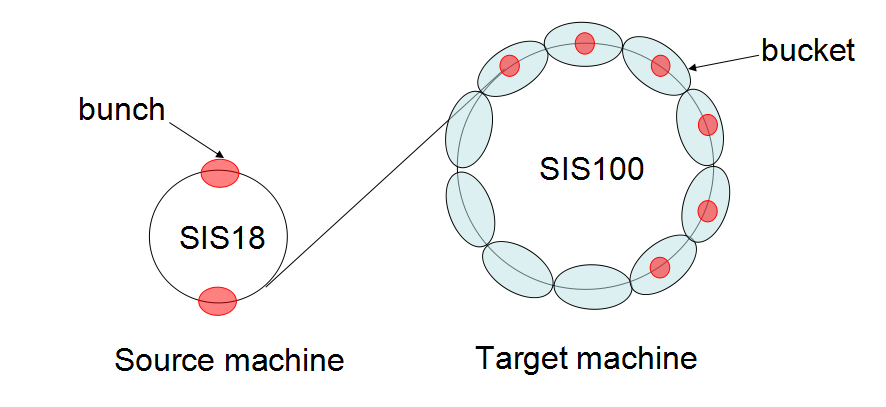
\includegraphics[width=85mm]{2to8.png}
%   \caption{The bunch to bucket transfer of U$^{28+}$ from the SIS18 to the SIS100.}
%   \label{fig1}
%\end{figure}
% 
%  For properly transferring the beam from the source synchrotron to the target synchrotron, the phase between the beam and the bucket must be precisely controlled before it is ejected. The process of achieving the detailed phase adjustment is termed "synchronization". There are mainly two methods to realize the synchronization: the phase shift and the frequency beating, both of which are based on the RF frequency modulation. To achieve the a required phase shift, the RF frequency is modulated away from the a nominal value for a period of time and then modulated back. The frequency beating is an comparison between two RF signals of slightly different frequencies, perceived as periodic variations in phase difference [0, 2$\pi$] whose rate is the difference between the two frequencies. 
%
%  We prefer to use the frequency beating method to realize the synchronization for the SIS18 and the SIS100, which has more synchronization chances compared with just once of the phase shift method. Fig.~\ref{fig2} shows the schematic of the synchronization process in one SIS18 cycle. A broad description of the synchronization process is as follows. On the RF ramp of the source synchrotron, the RF frequency de-tune is achieved. After receiving the timing event (e.g. "Synchronization begin") from the timing network, the TR which is coupled to the RF system then informs the RF device to collect information, including the RF frequency, the harmonic number, the phase difference between the RF signal and the reference signal and the timestamp of the zero crossing point of RF signal h = 1. After collection data, the RF device transfers data to the TR. Then the TR sends data to the TR of the SIS100 via the timing network. At the same time, the SIS100 does the same procedures. Until now, both synchrotrons have all information for the synchronization so that they are able to calculate the propagation of uncertainties~\cite{error_propogation} of the phase difference measurement, the coarse window. Besides, both synchrotrons resynchronize the RF signals of each other locally. With the help of the coarse window and the resynchronized RF signals, both synchrotrons trigger their kickers with precision better than 0.5$^\circ$, which makes the RF frequency beating method possible.
%
%\begin{figure}[!htb]
%   \centering
%   \includegraphics*[width=90mm]{sketch.png}
%   \caption{The schematic of the synchronization process in one SIS18 cycle.}
%   \label{fig2}
%\end{figure}
%
%  This paper, does not contain a detailed technical description of the synchronization process, rather is devoted to demonstrating the RF frequency de-tune from the viewpoint of beam dynamics and the theory of the frequency beating method instead, especially focusing on the bunch to bucket transfer from the SIS18 to the SIS100.
%
%
%
%\section{\label{sec:level1}Beam-dynamics view of the Frequency De-tune}
%
%  The first step for the bunch to bucket transfer is the RF frequency de-tune. In order to realize the frequency beating between two synchrotrons, the RF frequency of the source synchrotron or the target synchrotron or both synchrotrons can be de-tuned. It means that the particles on the de-tuned synchrotron run at an average radius different by $\bigtriangleup$R from the designed orbit R. For the synchronization of the SIS18 and the SIS100, we will de-tune the RF frequency on the SIS18. The SIS18 operates with a cycle length of 520ms, harmonic number of 2 ( h = 2 ), and RF frequency of approximately 0.43 MHz at injection and approximately 1.57 MHz at ejection for the $U^{28+}$~\cite{SIS18}. During nominal operation, the SIS18 forms two bunches from the beam injected at 11.4 MeV/$\mu$ and accelerates them up to 200 MeV/$\mu$. From the SIS18, 4 batches, each of 2 bunches, are transferred at  maximum 10ms intervals to the SIS100. The harmonic number of the SIS100 is 10 and the SIS100 RF frequency is fixed at approximately 1.57 MHz during the
%injection period to simplify the RF control system and to avoid perturbing batches already transferred.
%
%  This RF frequency de-tune is done accompanying with the RF ramp. Accepting to decentre the orbit by 8mm for the SIS18~\cite{SIS18_man}: 
%
%\begin{equation}
%\frac{\bigtriangleup{R}}{R}\approx{2.4}{\times}10^{-4}\label{eq1}
%\end{equation}
%
%  We know the basic differential relations among the fractional change in the RF frequency f, the fractional change in the momentum p, the fractional change in the bending magnetic field B and the fractional change in the radius R as follows ~\cite{J-PARC}.
%
%
%\begin{equation}
%\label{eq:eq2}
%\frac{\Delta{f}}{f} ={\frac{1}{\gamma^2}}{\frac{\Delta{p}}{p}} - \frac{\Delta{R}}{R}
%\end{equation}
%
%\begin{equation}
%\frac{\Delta{f}}{f} = (\frac{1}{\gamma^2}-\frac{1}{\gamma_t^2})\frac{\Delta{p}}{p}+{\frac{1}{\gamma_t^2}}{\frac{\Delta{B}}{B}}
%\label{eq:eq3}
%\end{equation}
%
%
%  where $\gamma$ is the relativistic factor, which measures the total particle energy, E, in
%units of the particle rest energy, $E_0$; $\gamma_t$ is the transition gamma; $\bigtriangleup{f}$ and  $\bigtriangleup{B}$ are the frequency and  bending magnetic field deviation for the frequency de-tune;  $\bigtriangleup{p}$ is the momentum deviation.
%
%  For J-PARC synchronizing the RCS (Rapid-Cycling Synchrotron)  with the MR (Main Ring) or the MLF (Materials and Life Science Facility), the RF phase shift of the RCS is adopted~\cite{J-PARC}. To achieve a required phase shift, the RF frequency is modulated away from the required value for a period of time and then modulated back, when the extraction and injection energy match again.  During its synchronization process, the magnetic field is not affected by the frequency change, namely $\Delta$B = 0. 
%
%  In our case of the frequency beating method, we guarantee the extraction and injection energy always match, which means that the momentum is not affected by the frequency change, namely $\Delta$p = 0; then the general relation between the radial excursion and RF frequency change Eq.~(\ref{eq:eq2}) reduces to Eq.~(\ref{eq:eq4}) and the general relation between the magnetic field change and RF frequency change Eq.~(\ref{eq:eq3}) reduces to Eq.~(\ref{eq:eq5}).
%
%\begin{equation}
%\frac{\Delta{f}}{f} = - \frac{\Delta{R}}{R}
%\label{eq:eq4}
%\end{equation}
%
%\begin{equation}
%\frac{\Delta{f}}{f} =  \frac{1}{{\gamma_t}^2}\times{\frac{\Delta{B}}{B}}
%\label{eq:eq5}
%\end{equation}
%
%From these equations, the RF frequency and the magnetic field change at the $U^{28+}$  extraction energy 200MeV/u~\cite{SIS18_man} ($\gamma_t$ = 5.8) are 
%
%\begin{equation}
%\frac{\Delta{f}}{f} = -{2.4}{\times}10^{-4}
%\label{eq6}
%\end{equation}
%
%\begin{equation}\frac{\Delta{B}}{B} = -{8.1}{\times}10^{-3}\label{eq5}
%\end{equation}
%
%where the maximum RF frequency de-tune is approximate to 370 Hz at 1.57 MHz for the $U^{28+}$. In this paper, we assume Rf frequency de-tune for the SIS18 equals to 200 Hz for the sake of simplicity.
%
%\section{\label{sec:level1}Synchronization of two machines}
%
%The second step for the bunch to bucket transfer is the synchronization of two synchrotrons using the frequency beating method. After the RF frequency de-tunes on the source synchrotron, the relative rf phase of the two synchrotrons begins to slip at a repetition rate of the absolute value of the difference in two RF frequency. When the correct amount of phase is accumulated, the bunch of the source synchrotron will align or be cogged with the bucket of the target synchrotron.
%
%\subsubsection{The test setup}
%
%Because the RF device is still under development, we use two MODEL DS345 Synthesized Function Generators~\cite{FG} with the frequency accuracy of $\pm$5 ppm of the selected frequency to simulate RF signals from RF cavities of the SIS18 and the SIS100. Two TRs, the FPGA-based cards, are responsible for the time/phase measurement, information transmission and coarse window calculation. (see Fig.~\ref{fig3})
%
%\begin{figure}[!htb]
%   \centering
%   \includegraphics*[width=90mm]{2pexaira.jpg}
%   \caption{The test setup for the bunch to bucket transfer.}
%   \label{fig3}
%\end{figure}
%
%\subsubsection{The frequency beating method}
%
%Here we still assume that the source synchrotron is the SIS18 and the target synchrotron is the SIS100. The RF frequency of the SIS18 is denoted by $f_{rf}^{SIS18}$ and that of the SIS100 by $f_{rf}^{SIS100}$. ${\bigtriangleup{f}}$ is the RF frequency de-tune value of the SIS18. n is the number of the SIS100 revolution period to realize the synchronization. $t_{18best}$ and $t_{100best}$ are the timestamps of the zero-crossing point of the RF signals measured by the TRs. According to the measurement results, there are two scenarios.
%
%\begin{itemize}
%    \item  $t_{18best} < t_{100best}$
%    \begin{equation}
%   t_{100best}+{n}\times{\frac{1}{f_{rf}^{SIS100}}}=t_{18best}+{(n+1)}\times{\frac{1}{(f_{rf}^{SIS18}+{\bigtriangleup{f}})}}
%   \end{equation}
%    \item  $t_{18best} > t_{100best}$
%    \begin{equation}
%   t_{100best}+{n}\times{\frac{1}{f_{rf}^{SIS100}}}=t_{18best}+{n}\times{\frac{1}{(f_{rf}^{SIS18}+{\bigtriangleup{f}})}}
%   \end{equation}
%\end{itemize}
%
%
%Based on these two scenarios, we could deduce the formulas for the number of the SIS100 revolution n and the time  $t_{syn}$ spend on the synchronization.
%
%\begin{equation}
%n=\frac{t_{100best}-t_{18best}-\frac{\bigtriangleup{n}}{f_{rf}^{SIS18}+{\bigtriangleup{f}}}}{\frac{1}{f_{rf}^{SIS18}+{\bigtriangleup{f}}}-\frac{1}{f_{rf}^{SIS100}}}\label{eq6}
%\end{equation}
%
%\begin{equation}
%t_{syn}=\frac{(f_{rf}^{SIS18}+{\bigtriangleup{f}})\times{t_{18best}}-f_{rf}^{SIS100}\times{t_{100best}}+{\bigtriangleup{n}}}{(f_{rf}^{SIS18}+{\bigtriangleup{f}})-f_{rf}^{SIS100}}\label{eq7}
%\end{equation}
%
%where $\bigtriangleup{n}$ equals 1 when  $t_{18best} < t_{100best}$ and equals 0 when  $t_{18best} > t_{100best}$.
%
%\subsubsection{The coarse window and an example}
%
%The coarse window is the result of the propagation of uncertainties of the phase difference measurements. The uncertainties in $f_{rf}^{SIS18}$, $f_{rf}^{SIS100}$, $t_{18best}$ and $t_{100best}$ are independent and random, then the uncertainty~\cite{error_propogation} in the synchronization time $t_{syn}$ is
%
%\begin{widetext}
%\begin{equation}
%\delta {t_{syn}}=\sqrt{(\frac{\partial{t_{syn}}}{\partial{t_{18best}}}{\delta{t_{18}}})^{2}+(\frac{\partial{t_{syn}}}{\partial{t_{100best}}}{\delta{t_{100}}})^{2}+(\frac{\partial{t_{syn}}}{\partial{f_{rf}^{SIS18}}}{\delta{f_{rf}^{SIS18}}})^{2}+(\frac{\partial{t_{syn}}}{\partial{f_{rf}^{SIS100}}}{\delta{f_{rf}^{SIS100}}})^{2}} 
%\label{eq:coarse}
%\end{equation}
%\end{widetext}
%
%
%After calculation, we get the result of $\delta$$t_{syn}$
%
%\begin{align*}
%&A=\frac{(f_{rf}^{SIS100})^2+(f_{rf}^{SIS18}+\bigtriangleup{f})^2}{\bigtriangleup{f}^2}\nonumber\\
%&B=\frac{2\times{[(f_{rf}^{SIS18}+\bigtriangleup{f})\times(t_{18best}-t_{100best})+{\bigtriangleup{n}}]^2}}{\bigtriangleup{f}^4}\nonumber\\
%&C=\frac{2\times{(f_{rf}^{SIS18}+\bigtriangleup{f})}\times(t_{18best}-t_{100best})^2}{\bigtriangleup{f}^3}+\nonumber\\
%&      \frac{2\times{\bigtriangleup{n}}\times(t_{18best}-t_{100best})}{\bigtriangleup{f}^3}\\
%&D=\frac{(t_{18best}-t_{100best})^2}{\bigtriangleup{f}^2}\nonumber\\
%\end{align*}
%\begin{equation}
%\delta {t_{syn}}=(A\times\delta{t}^2+B\times\delta{f}^2-C\times\delta{f}^2+D\times\delta{f}^2)^{\frac{1}{2}}\label{eq8}
%\end{equation}
%
%where we assume that $f_{rf}^{SIS18}$=$f_{rf}^{SIS100}$ = 1.57 MHz, the RF frequency of the flattop of the SIS18 and of the injection of the SIS100 for the $U^{28+}$, $\bigtriangleup{f}$=200 Hz. In the real situation, the uncertainty of the phase difference measurement from the RF device is 50 ps, $\delta$$t_{18}$ = $\delta$$t_{100}$ = $\delta{t}$ = 50 ps. Because the RF frequency has the long term stability in the real RF system, $\int\delta{f_{rf}^{SIS18}}dt$ = $\int\delta{f_{rf}^{SIS100}}dt$ = 0. 
%
%Based on these assumptions, the coarse window is $\pm$\unit[0.55][$\mu$s] of the best estimation. The maximum time for the synchronization is 
%
%
%\begin{equation}
%\frac{1}{\Delta{f}} = \frac{1}{200 Hz} = 5 ms\label{eq9}
%\end{equation}
%
%Based on this window, we make use of the first SIS100 revolution signal after the $t_{syn}$ - 0.55us and the following SIS18 revolution signal to trigger kickers. In order to guarantee that each bucket has opportunity to be injected, the whole period of the first SIS100 revolution signal is available. So the accuracy within this period is better than 0.5$^\circ$
%
%\begin{equation}
%{\frac{6.4 \mu s}{5ms}}\times {360^\circ} \approx 0.46^\circ\label{eq9}
%\end{equation}
%
%Where 6.4 $\mu$s is the revolution period of the SIS100.
%\begin{equation}
%\frac{1}{f_{rf}^{SIS100}}\times {h} = \frac{1}{1.57 MHz}\times {10} = 6.4 \mu s \label{eq10}
%\end{equation}
%
%\subsubsection{Test result}
%This setup theoretically simulates the synchronization of two synchrotrons, with accuracy better than 0.5$^\circ$ (see Table~\ref{tab:table1}). It paves the way for the further FAIR bunch to bucket transfer. \\
%
%\begin{table}[]
%\caption{The test result of the bunch to bucket transfer}
%\begin{ruledtabular}
%\begin{tabular}{ll}
%\label{tab:table1}
%Bunch to Bucket Transfer of  $U^{28+}$ from SIS&18 to SIS100\\
%\hline
%SIS18 RF frequency ( h = 2 )& 1.57 MHz \\
%SIS100 RF frequency ( h = 10 ) & 1.57 MHz\\
%
%The RF frequency de-tune of SIS18 & 200 Hz\\
%The phase difference in the time domain & 577 ns\\
%The number of SIS100 revolution for\\  the synchronization ( n ) & 7112\\
%
%The time consumption for the \\  synchronization & 4.530 ms\\
%
%The synchronization period & 5 ms\\
%The coarse window  & 0.56 $\mu s$\\
%The accuracy within one SIS100\\  revolution period  & 0.45$^\circ$\\
%
%\end{tabular}
%\end{ruledtabular}
%\end{table}
%
%\section{\label{sec:level1}Summary}
%The frequency beating method based on the RF frequency de-tune realizes the synchronization process between the SIS18 and the SIS100. It will be used for the synchronization of other machines for FAIR, such as the synchronization between the SIS18 and the ESR, the CR and the HESR and so on. 
%
%\begin{acknowledgments}
%The author would like to thank all staff in the department of control systems of GSI for their patient guidance, enthusiastic encouragement and useful critiques of the research work. The author would also like to thank staff from the Department Ring RF Systems to provide useful information about the RF system. The grateful thanks are also extended to Peter Moritz for his support.
%\end{acknowledgments}
%
%\appendix
%
%\section{The parameters related to the bunch to bucket transfer from the SIS18 to the SIS100}
%\begin{table*}
%\caption{\label{tab:table3}All parameters related to the bunch to bucket transfer for Radioactive Ion Beam (RIB) from the SIS18 to the SIS100}
%\begin{ruledtabular}
%\begin{tabular}{lccc}
%&&RIB\\ \hline
%&&SIS18 Extraction&SIS100 Injection\\ \hline
%Designed Orbit&m&216.72&1083.6\\
%Extraction kinetic energy&Mev/u&200&\\
%Injection kinetic energy&Mev/u&&200\\
%RF harmonic &&2&10 ({2 bunch}$\times${4 batches})\\
%RF frequency&MHz&1.572&1.572\\
%RF period&$\mu$s&0.636&0.636\\
%Revolution frequency&MHz&0.786&0.157\\
%Revolution period&$\mu$s&1.272&6.359\\
%$\beta$&&0.568&0.568\\
%$\gamma$&&1.215&1.215\\
%Transition energy $\gamma_t$&&5.8&\\
%Momentum compaction $\alpha_p$&&0.030&\\
%$\Delta$R/R&&{$\pm$2.4}$\times{10^{-4}}$&\\
%Max $\Delta$f/f&&$\pm$0.024$\%$&\\ 
%$\Delta$p/p&&&1$\%$\\ \hline
%&&Synchronization process\\ \hline
%Beating frequency&MHz&1.572+0.2&1.572\\
%Frequency difference&Hz&200\\
%Synchronization period&$\mu$s&5&5\\
%$\Delta$f/f by the frequency de-tune&&0.013$\%$&\\
%
%Injection precison&&&better than $1^o$\\
%
%
%\end{tabular}
%\end{ruledtabular}
%\end{table*}
%
%
%\begin{thebibliography}{99} 
%
%\bibitem{GMT_system}
%	D. Beck, R. B$\ddot{a}$r, M. Kreider, C. Prados, S. Rauch, W. Terpstra and M. Zweig ,
%	\textit{THE NEW WHITE RABBIT BASED TIMING SYSTEM FOR THE FAIR FACILITY},
%	PCaPAC'12, India, p.~242, (2012)
%
%\bibitem{GMT_BuTiS}
%	D. Beck, 
%     \textit{Interface to BuTiS},
%	\url{https://www-acc.gsi.de/wiki/Timing/TimingSystemButisInterface}
%
%\bibitem{WR}
%	D. Beck, R. B$\ddot{a}$r, T. Fleck, M. Kreider, S. Mauro, C. Prados, S. Rauch, W. Terpstra and M. Zweig, 
%     \textit{White Rabbit Technology as Basis for the FAIR Timing System}
%	GSI Scientific Report 2011, p.~333, (2011)
%
%\bibitem{BuTis}
%	P. Moritz,
%	\textit{BuTiS - Development of a Bunchphase Timing System},
%	GSI Scientific Report 2006, p.~64, (2007)
%
%\bibitem{batch}
%	G. Dugan,
%	\textit{Considerations of BunchSpacing Options for Multi-Bunch Operation of the Tevatron Collider},
%	Fermi National Accelerator Laboratory, p.~1, (1989)
%
%
%\bibitem{SIS18_100}
%     D. Ondreka,
%	\textit{Settings Generation for the RF Systems in FAIR},
%	GSI/CERN Meeting 2014
%
%\bibitem{SIS18_man}
%     H. Liebermann, D. Ondreka,
%	\textit{FAIR and GSI Reference Cycles for SIS18},
%	GSI, October 3, 2013
%
%\bibitem{J-PARC}
%     Eizi EZURA, Masahito YOSHII,
%	\textit{BEAM-DYNAMICS VIEW OF RF PHASE ADJUSTMENT FOR SYNCHRONIZING J-PARC RCS WITH MR},
%	High Energy Accelerator Research Organization, Japan, June, 2008
%
%\bibitem{error_propogation}
%    John R. Taylor,
%    \textit{AN INTRODUCTION TO Error Analysis} 
%    University Science Books, Sausalito, California, 1997
%
%\bibitem{SIS18}
%    H Liebermann, D. Ondreka,
%    \textit{FAIR and GSI Reference Cycles for SIS18} 
%    Primary Beams - System Planning, Sausalito, GSI, 2013 
%
%\bibitem{FG}
%     Stanford Research Systems,
%	\textit{MODEL DS345 Synthesized Function Generator}
%
%\bibitem{DSP}
%      H. Klingbeil,
%      \textit{Low-Level-RF (LLRF) Systems for FAIR Synchrotron and Storage Ring Cavities},
%      FAIR-Technikforum, November.11.2010
%\addtocounter{enumi}{5}
%
%
%\end{thebibliography}


\end{document}

